\documentclass[12pt,a4paper,twoside]{report}         
\usepackage{cs}              
\usepackage{times}
\usepackage{graphicx}
\usepackage{latexsym}
\usepackage{amsmath,amsbsy}
\usepackage{amssymb}
\usepackage[matrix,arrow]{xy}
\usepackage[T1]{fontenc}
\usepackage{ae,aecompl}
\usepackage{amstext}
\usepackage{graphics}
\usepackage[T1]{fontenc}
\usepackage{ae,aecompl}
\usepackage{algorithm}
%\usepackage{algorithmic}
\usepackage{listings}
\usepackage{color}
\usepackage{color}
\usepackage{float}
\diplomathesis
\centerchapter
\singlespace
\setcounter{secnumdepth}{3}

\renewcommand{\thesisauthor}{Paul Tudor LINCA}
\renewcommand{\thesismonth}{July}
\renewcommand{\thesisyear}{2020}
\renewcommand{\thesistitle}{FlickRank} 
\renewcommand{\thesissupervisor}{Assist. Prof. Dr. Eng. Ion GIOSAN}
\newcommand{\department}{\bf FACULTY OF AUTOMATION AND COMPUTER SCIENCE\\
COMPUTER SCIENCE DEPARTMENT}
\newcommand{\thesis}{LUCRARE DE LICEN'T'A}
\newcommand{\utcnlogo}{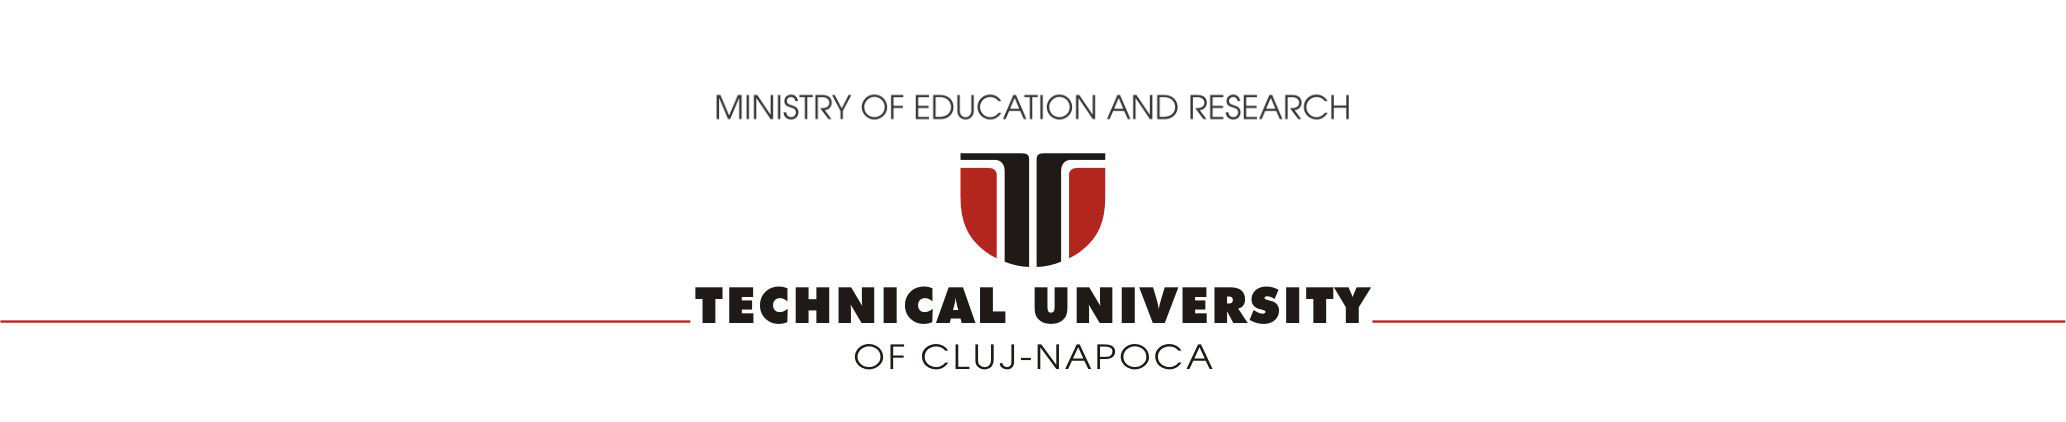
\includegraphics[width=15cm]{img/tucn.jpg}}

\newcommand{\uline}[1]{\rule[0pt]{#1}{0.4pt}}
%\renewcommand{\thesisdedication}{P\u{a}rin\c{t}ilor mei}

\begin{document}
%\frontmatter
%\pagestyle{headings}

\newenvironment{definition}[1][Defini\c{t}ie.]{\begin{trivlist}
\item[\hskip \labelsep {\bfseries #1}]}{\end{trivlist}}



%\thesistitle                    %% Generate the title page.
%\authordeclarationpage                %% Generate the declaration page.


\begin{center}
\utcnlogo

\department

\vspace{4cm}

\textbf{REVIEW AGGREGATION APPLICATION\\USING WEB CRAWLING AND IMAGE PROCESSING }

\vspace{1cm}

LICENSE THESIS

\vspace{7cm}

Graduate: {\bf \thesisauthor} 

Supervisor: {\bf \thesissupervisor}

\vspace{2cm}
{\bf \thesisyear}

\end{center}

\thispagestyle{empty}
\newpage

\begin{center}
\utcnlogo

\department

\end{center}
\vspace{0.5cm}

\begin{tabular}{p{7cm}p{8cm}}
 %\hspace{-1cm}& APPROVED,\\
 \hspace{-1cm}DEAN, & HEAD OF DEPARTMENT,\\
 \hspace{-1cm}{\bf Prof. dr. eng. Liviu MICLEA} & {\bf Prof. dr. eng. Rodica POTOLEA}\\  
\end{tabular}
 
\vspace{2cm}

\begin{center}
Graduate: {\bf \thesisauthor}

\vspace{1cm}

{\bf REVIEW AGGREGATION APPLICATION\\USING WEB CRAWLING AND IMAGE PROCESSING}
\end{center}

\vspace{5mm}

\begin{enumerate}
 \item {\bf Project proposal:} {\it Develop an Android application that provides the user a way to search for a desired movie, either manually or by taking a photo of its poster, and gathers its reviews from various sources. }
\item {\bf Project contents:} {\it  Introduction, Project Objectives and Specifications, Bibliographic Research, Analysis and Theoretical Foundation, Detailed Design and Implementation, Testing and Validation, User’s Manual, Conclusions, Bibliography.}
\item {\bf Place of documentation:} Technical University of Cluj-Napoca, Computer Science Department
\item {\bf Consultants:} {\it \thesissupervisor}
\item {\bf Date of issue of the proposal:} {\it November 1, 2019}
\item {\bf Date of  delivery:} {\it July 8, 2020}
  \end{enumerate}
\vspace{1.2cm}

\hspace{6cm} Graduate: \thesisauthor

\vspace{0.5cm}
\hspace{6cm} Supervisor: \thesissupervisor

\thispagestyle{empty}


\newpage

\begin{center}
\utcnlogo

\department
\end{center}

\vspace{0.5cm}

\begin{center}
{\bf
Declara\c{t}ie pe proprie r\u{a}spundere privind\\ 
autenticitatea lucr\u{a}rii de licen\c{t}\u{a}}
\end{center}
\vspace{1cm}



Subsemnatul \thesisauthor, legitimat cu buletin seria CJ nr. 459435 CNP 1980108260038, autorul lucr\u{a}rii "Review Aggregation Application Using Web Crawling and Image Processing" elaborat\u{a} \^{\i}n vederea sus\c{t}inerii examenului de finalizare a studiilor de licen\c{t}\u{a} la Facultatea de Automatic\u{a} \c{s}i Calculatoare, Specializarea CTI Engleza din cadrul Universit\u{a}\c{t}ii Tehnice din Cluj-Napoca, sesiunea Iulie a anului universitar 2019/2020, declar pe proprie r\u{a}spundere, c\u{a} aceast\u{a} lucrare este rezultatul propriei activit\u{a}\c{t}i intelectuale, pe baza cercet\u{a}rilor mele \c{s}i pe baza informa\c{t}iilor ob\c{t}inute din surse care au fost citate, \^{\i}n textul lucr\u{a}rii \c{s}i \^{\i}n bibliografie.

Declar, c\u{a} aceast\u{a} lucrare nu con\c{t}ine por\c{t}iuni plagiate, iar sursele bibliografice au fost folosite cu 
respectarea legisla\c{t}iei rom\^{a}ne \c{s}i a conven\c{t}iilor interna\c{t}ionale privind drepturile de autor.

Declar, de asemenea, c\u{a} aceast\u{a} lucrare nu a mai fost prezentat\u{a} \^{\i}n fa\c{t}a unei alte comisii de examen de licen\c{t}\u{a}.

\^{I}n cazul constat\u{a}rii ulterioare a unor declara\c{t}ii false, voi suporta sanc\c{t}iunile administrative, respectiv, \emph{anularea examenului de licen\c{t}\u{a}}.

\vspace{1.5cm}

\hspace{9cm} Nume, Prenume

\vspace{0.5cm}

8 Iulie, 2020 \hspace{6.5cm} \thesisauthor

\vspace{0.5cm}

\thispagestyle{empty}

\newpage

\pagenumbering{roman}
\setcounter{page}{1}

\newpage

\tableofcontents
\newpage

\pagenumbering{arabic}
\setcounter{page}{1}

\chapter{Introduction}
%=======================================================================================================
\section{Project context}

“Time is money” is an expression everybody has heard before. It refers to the
fact that time is one of the most valuable resources man possesses and that it
should be spent doing things that improve one’s life instead of trivial actions.
This introduces a critical problem humanity faces, one that is responsible for
most of people’s wasted time: decision making.

Decision making represents one of the most wasteful actions we, humans, do.
Questions like “What to wear?”, “Where to eat?” are ones that everybody faces
on a daily basis. Another major one is “What to watch?”. Due to the sheer
amount of choices available, deciding on a single movie to watch is an obstacle
that should be removed in order to boost one’s productivity. Having said that,
the best way to decide if a movie is a great fit is its reviews and reading other
people’s opinions on it.

On the other hand, there's a noticeable growing emphasis on convenience for today's population. According to the NRF (National Retail Federation) [1], there's a significant change in how consumers decide which product to use now. While price and quality still top the chart of what matters the most when choosing a service, convenience has seen a considerable increase over the past few years. This places it at the number 3 spot, slowly advancing its way up.

Circling back to our problem, while we established that reviews are the most influential factor when choosing a movie to watch, the inconvenience of sifting through the various review websites there are, often alienate people from actually reading them.

My project illustrates how time efficiency and convenience are aspects of life that can be significantly boosted by various techniques.

\newpage
%=======================================================================================================

%=======================================================================================================
\section{Domain Specification}

There are three major domains that are encompassed in my project are Android mobile development, web scraping and image processing.

% Why Android?

With over 1.6 billion users and maintaining over 70\% of the mobile operating system global market share [2], the Android OS is undoubtedly the best choice for running and developing my application. Android is an operating system, based on the Linux kernel, designed primarily for mobile devices. It is designed and developed by Google. On May 7, 2019, Google replaced Java as its preferred language for Android app development with Kotlin. Due to its increasing popularity and abundant tools and resources, the mobile application of my project will be developed using Kotlin with the Android Studio IDE.

% Why Web scraping?

In simple terms, web scraping can be described as a system that allows mass browsing and/or downloading of web pages. While it can be done manually by a user, the process is usually automated by implementing a web crawler. Also called "bots", "spiders" or simply "crawlers", web crawlers are typically used for extracting data from websites in order to use it for other purposes. Due to its ability to retrieve targeted data from multiple sources automatically and swiftly, web crawling will be the backbone of the movie review aggregation aspect of my project.

% Why image processing?

Image processing is a field of computer science that primarily deals with creating functions and algorithms that accept images as input. Images are defined by two dimensions, coming together to form pixels. Thus, image processing is the act of performing some actions in a particular order, for the sake of building an enhanced image or extracting useful information from it. Nowadays, image processing is one of the most profitable and growing technologies. One only has to look at the popularity of Instagram and other image sharing platforms in order to comprehend the importance and scale of the industry. Of course, more practical use cases for it do exist, which are included in domains such as medicine, chemistry, physics, astrology, security and many more. That being said, we could draw the conclusion that image processing is one of the most efficient tools for boosting convenience and automating time consuming tasks. 

% APIs

In order for these three giants to be able to work together, an API will be used. APIs or "Application Programming Interfaces" have changed the way mobile applications are developed and used by allowing them to interact with other components. They single-handedly boosted how apps get integrated and communicate. Some would say they are the "hidden backbone" [3] of the modern world. In simple terms, they expose the internal functions and services of a program to the outside world, for any other program with the correct permissions to use. One could say that most, if not all, of the apps that are successful today make use of APIs. Thus, it goes without saying that my project will benefit from using one or more APIs in order to achieve its goals.

%=======================================================================================================  

\chapter{Project Objectives and Specifications}

%=======================================================================================================  

This chapter of the documentation will present the objectives, specifications and proper motivation for the project.
\section{Project Overview}

The main purpose of this project is to build an Android mobile application that allows users to: search for a specific movie, by either manually typing the title or taking a photo of its poster, view the details about the movie, see reviews of the movie from numerous sources, browse through recommendations that are based on recently viewed films. The application will make use of existing APIs, but will also make use of a project specific API. 

The API developed in the context of this project, will deliver the client with: reviews of a specific movie, by means of web scraping, movie recommendations, lists of what movies are currently popular and movie titles based on their posters.

The end goal of my project is to help its users reach a decision quicker. Image search provides a faster alternative to manually typing, while the review aggregation aspect of the application exempts the user from endlessly browsing websites, saving them a lot of clicks and, implicitly, time. All this put together should aid the user in answering the following questions:
    \begin{itemize}
        \item "What movie should I watch?"
        \item "Is this movie good?"
        \item "Is this movie a good match for me?"
        \item "What movies are popular today?"
        \item "What movies are similar to this movie?"
    \end{itemize}
    
%=======================================================================================================  

%=======================================================================================================  
\section{Goals and Objectives}

The project consists of three main goals: building an Android application from scratch, implementing a fast and reliable web scraper and developing a poster recognition program. Each one of the three main goals represent pretty complex and high order tasks. Thus, breaking them down into smaller sub-tasks, as well as scheduling them correctly will increase the efficiency and speed of the overall project development process.

\subsection{Task \& Progress Tracking}

As I want to be as efficient as possible, which will also reflect on the overall quality of the project, the goals, tasks and sub-tasks of the project must be tracked properly. For this, I decided to use Jira.

Jira is, essentially, a work management tool, mostly used for software development. It was developed by Atlassian to allow development teams to create detailed tasks and reminders, assign them to specific team members, see the overall progress of a project, track bugs and issues and much more. 

Jira provides many popular management tools. One such tools is the Kanban board. It is used to help visualize work, help prioritize assignments, provide a better view of the work-flow and, at its core, maximize efficiency. It is composed of numerous columns, each one representing an activity. All of the columns together make up the workflow of the project. 

\begin{figure}[H]
    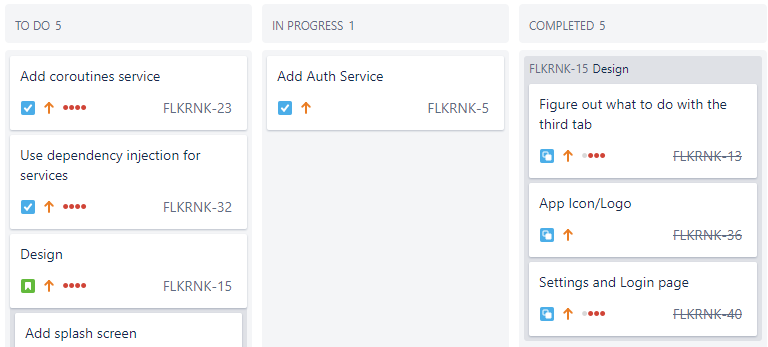
\includegraphics[width=\textwidth]{templateLaTeX-Eng/img/kanbanboard.png}
    \caption{\bf Snippet of the project's Kanban board in Jira}
\end{figure}

Most, if not all, tasks that get created start off in the first column, in my case, the "To Do" column. Tasks can be broken down into smaller sub-tasks and be ordered by their level of priority. High priority tasks will appear at the top of the column. A "Work In Progress" limit will be added so that I can focus on a single task at a time and not get overwhelmed. When I choose a task for development, it will be positioned in the "In progress" column. At completion, the task will be set on the "Done" column.

I believe having a visual representation of the development flow of any project greatly enhances productivity and quality. Besides being very intuitive and easy to understand, Jira and its Kanban board have saved me a great amount of time and stress. Actually seeing the progress of a project has been proved to remarkably increase productivity and morale.

\subsection{Research}

In order to not rush and overload the project, research on each subject must be done. This means finding best suited technologies and methodologies for what I am trying to achieve. The research process will result in a clear understanding of the best practices and procedures that I should follow in order to make development as smooth as possible. Research must be done on technologies, programming languages, frameworks, architectures, tools and existing libraries or APIs. This section will be described in more detail in chapter 3.

\subsection{Main Goals}

\begin{enumerate}
    \item Design and develop an intuitive, appealing and fast Android mobile application that aggregates movie reviews from various sources.
    \item Implement an image processing program that receives as input an image that contains a movie poster, and outputs the name of the movie.
    \item Create a web scraper that searches the web for reviews of a particular movie and aggregates them in a common format.
\end{enumerate}

\noindent These goals are a great starting point for developing the application but do not necessarily work as standalones. Thus, another goal can be defined:

\begin{enumerate}
    \setcounter{enumi}{3}
    \item Create an API that exposes the functionalities of 2 and 3 in its endpoints and deploy it so it can be accessed publicly.
\end{enumerate}

Now that the main objectives have been established, they must be broken down into smaller steps. As said before, this will make the development process more manageable and seem more achievable.

\newpage

\subsection{Breakdown of the Main Goals}

\begin{enumerate}
    \item Android application:
    \begin{itemize}
        \item Research best practices, architecture, libraries and choose the best approach.
        \item Build a prototype with basic functionality.
        \item Add user authentication.
        \item Properly implement each separate functionality, while also integrating the used APIs.
        \item Give the application a proper design and UI.
    \end{itemize}
    \item Poster recognizer:
    \begin{itemize}
        \item Detect and extract the poster from the input picture.
        \item Perform a four perspective transform on the extracted poster.
        \item Gather a collection of movie poster for comparison.
        \item Apply comparison operations between the extracted poster and the comparison ones.
        \item Choose the best match.
    \end{itemize}
    \item Review scraper: This can simply be broken down into smaller web scrapers for each desired source and then encompass them into a web scraping wrapper
    \item API:
    \begin{itemize}
        \item Research and choose the best suited framework for development.
        \item Create endpoints for each desired functionality.
        \item Run and test locally.
        \item Integrate the API into the Android app.
        \item Deployment.
    \end{itemize}
\end{enumerate}

%======================================================================================================= 
\section{Performance and requirements}

Performance is a key factor in today's mobile app market. Research suggests that users are very unforgiving when it comes to mobile application performance and consistence [4]. Quite a lot of mobile users discard apps when they take a considerable amount of time to load and never look back. After all, one could argue that the whole point of mobile devices is to provide access to data as fast as possible.

\subsection{Functional Requirements}
\noindent The functional requirements for mobile applications can simply be broken down into features:
\begin{itemize}
    \item The user should be given the option to authenticate into the application without creating a new account. This means accounts on other platforms could be linked to the system in question.
    \item The application should provide both manual and image search.
    \item The application should have data about most, if not all, movies.
    \item The system should fetch reviews from at least one source for each movie.
    \item The user should receive recommendations based on their watch preferences.
\end{itemize}

\subsection{Non-functional Requirements}
\begin{itemize}
    \item \textit{Performance:} As stated before, performance is the most important requirement. The user should be able to log into the application and find the reviews of the desired movie in a minimal amount of taps and time. Thus, a the amount of taps one would need to make shouldn't go above 7 and it shouldn't take more than 15 seconds. Load time for any page shouldn't exceed 5 seconds.
    \item \textit{Scalability:} As the amount of users increases, the system shouldn't have to jeopardize performance in order to "accommodate" them. Thus, the system API should initially be able to handle 10000 requests at any time.
    \item \textit{Responsiveness:} The application should be responsive to user input. Text fields, buttons and other input components shouldn't get stuck or not give feedback when the user interacts with them. Also, the application should be able to return to the same state in the case of an unexpected interruption (i.e. the user gets a call).
    \item \textit{Use-ability:} There is a common saying: "Less is more", which also applies to mobile app development. This means that the application should be as minimalistic and simple as possible so that any user would be able to use it without any problems.
    \item \textit{Security:} All app data and user sensitive data should be encrypted and secured such that it is protected from outside and inside attacks. Authentication should be secure and the authentication token should be saved properly.
    \item \textit{Availability:} The application should be available to anyone and users should be able to install, update and give feedback easily. Solving this is pretty straight forward. As most apps, this will be available on the Google Play Store. Also, the API will be deployed on a very reliable platform.
    \item \textit{Screen Adaptation:} As there is a wide variety of Android mobile devices, screens come in all shapes and sizes. The app should be able to render all its page layouts on all screens without altering much of the intended design. Fonts and images should be adjusted accordingly.
\end{itemize}

%=======================================================================================================  

\chapter{Bibliographic research}

%=======================================================================================================  

\section{Introduction}

Decision making is a major aspect of our day to day lives. It is present in most of our daily activities, from food intake to entertainment consumption. It involves a choice between alternatives. As the set of options grows, the harder the decision process, leading to one critical problem. 

As we all know, reaching a decision takes time. It was mentioned in the opening of this paper that time is one of the most valuable resource we possess and people have started being aware of this, now more than ever. Nowadays, society has been growing more addicted to a faster paced lifestyle which has lead to a significant increase in decision making on a whim. 

Authors Yoel Inbara, Simona Bottib, Karlene Hankoc have done extensive research [5] on human decision making that points towards the fact that larger choice sets often lead to greater regret, proposing that people apply the lay theory that “a quick choice is a bad choice” when evaluating how well they have chosen. This was also pointed out by Kathleen L. Mosier, Linda J. Skitka [6] who have reached the conclusion that automated decision aids have become more and more popular in our era. Speeding up the decision making process is one of the main objectives of my project and directly aligns with the research done by the authors mentioned above.

From Dr. Eugene J. Kelly's paper on convenience [7], it can be seen just how important commodity and convenience is for customers and users. He even identified 10 convenience forms in the context of consumer behavior. That's even more impressive when you take into account that the paper was first published in 1958. Nowadays, people will pay more for the more convenient option.

This project tackles the problem of decision making in the context of media consumption, in particular, movie watching choices. With an astounding \$136  billion net worth, the movie industry plays a major role in today's world. The following sections will contour numerous procedures that, assembled together, will provide users a convenient method for reaching a decision quicker when choosing a movie to watch.

%=======================================================================================================  

%=======================================================================================================  

\section{Poster recognition}

\subsection{Image Processing}

Even though image processing is a relatively recent field, there is a noticeable demand for applications that implement solutions using such methods. The domains that benefit from numerous variations of image processing are vast and diverse. From data security to biomedical imaging, the applications of this technology are never ending. Basically, whatever application has information that can be represented though images, can benefit have a lot to gain from this field. Thus, the attention that image processing has received over the past few years is not surprising. 

John C. Russ simply defined image processing in his book [8], as operations and methods that start with an image and end with an image. Images can be broken down into an array of pixels, each with its own information about brightness value or color aspects. Additionally, by applying numerous of the previously mentioned operations in a specific order, several new and useful pieces of information can be extracted, that otherwise couldn't be reached. This is one of the major advantages image processing provides.

Another major advantage is something that Google already capitalized on ages ago. The Google Search algorithm was totally changed for the better with the introduction of the image search. With their new and efficient image processing algorithms, users have been benefiting from faster and more convenient searches for a while now. The removal of the need to type words in and using images as a search query introduced by Google, is the one of the main inspirations for my project.

It is clear that the desired functionality of searching a movie by taking a photo of its poster can be achieved  though various techniques of image processing. 

\subsection{OpenCV}

OpenCV is an open source library that is concerned with image and video analysis. It was initially developed and introduced by Intel in 2000. Since then, many programmers have contributed towards its evolution.  With over 2500 optimized algorithms, 2.5 million downloads and over 40 thousand people in the user group [9], OpenCV is one of the most popular image processing libraries in use today.

The OpenCV library is divided into numerous modules, each mainly dedicated to a specific area of concern in the field of computer vision. It also provides various classes for representing data. The most used, perhaps, is the class Mat. As the name suggests, it essentially is a matrix that contains pixel values of images and other useful attributes.

Even though the library is written in C++ and its main interface is in C++, bindings in Python, Java and even MATLAB exist. Additionally, a lost of wrappers for other languages have been developed, such as C\#, Ruby, Perl and Haskell. Each option is thoroughly documented and a lot of online resources can be found for each.

\subsection{Edge Detection}

Users cannot be trusted when providing input, more so when it comes to images. Not everyone is photography savvy so user submitted images can have a lot of extra information. Thus, we can assume that the input images may contain other objects other that the poster. This results in the first step in our poster recognition process: the detection of the poster itself.

The approach employed by P. Shopa, N. Sumitha, P.S.K Patra in their paper [10], for traffic sign detection, is a fairly popular one. Canny edge detection is one of the most popular edge detection algorithms. It's no wonder that the previously mentioned authors decided to use it in their project. Of course, before actually performing John F. Canny's algorithm, a few extra pre-processing steps were taken. The color input image was first converted to grayscale and then thresholded, resulting in a black and white image. For an enhanced detection, a Gaussian filter was applied to the image as well. It can be seen in the figure below, that their results are satisfactory.

\begin{figure}[H]
    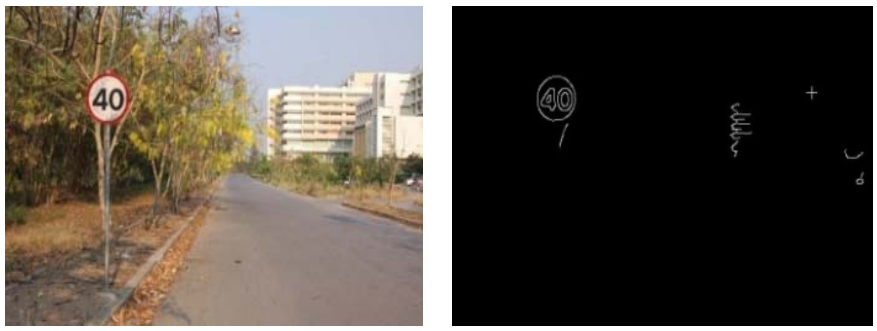
\includegraphics[width=\textwidth]{templateLaTeX-Eng/img/cannytrafficsigns.png}
    \caption{\bf Edge detection performed in [10]}
\end{figure}

Of course, all we have now is a black and white image. No actual information about the edges is explicitly known. Fortunately, OpenCV has an in-built function that finds the contours of an image and returns a structure containing the contours as an array of points, as well as their hierarchy. Guobo Xie and Wen Lu used a similar approach in their paper [11] as the formerly mentioned authors. They displayed their results neatly, clearly differentiating each contour using colors.

\begin{figure}[H]
    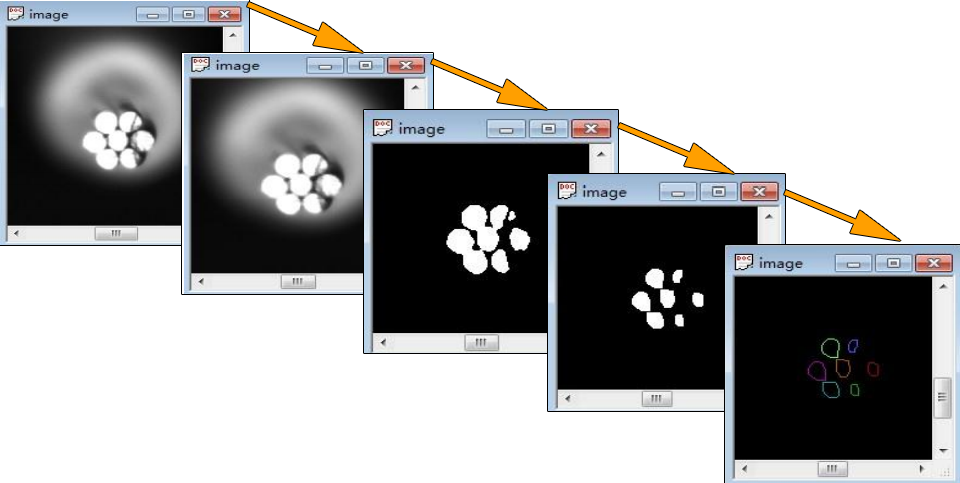
\includegraphics[width=\textwidth]{templateLaTeX-Eng/img/11pipeline.png}
    \caption{\bf Edge detection pipeline employed by Guobo Xie and Wen Lu in [11]}
\end{figure}

\subsection{Poster extraction}

The next logical step is to examine the contours and determine which one is the poster, after which, a perspective transformation must be applied.

Matthew Russell and Scott Fischaber used the Ramer-Douglas-Peucker algorithm to approximate shapes in their traffic sign detection project [12]. The algorithm essentially breaks down curves into points. The number of the resulting points would suggest what shape the contours form. In our case, posters are rectangles, thus, if the algorithms returns four points, that means that it would most likely be a poster.

Adrian Kaehler and Gary Bradski highlight a very useful function present in the OpenCV repertory in their book [13]. The perspective transform function is a special function that performs various perspective transformation over lists of points. This would boost our skewed input poster into a properly rectangular image that is perfect for comparison with original posters.

\subsection{Image comparison}

The problem of retrieving images that are similar to an input image is a very old issue. After all, this is the main functionality of image search engines. Many solutions currently exist, from easy to complex ones. 

As Kenneth Dawson-Howe describes in his book [14], a first step in image comparison would be to analyze the color distribution in the images. This would be done by computing their histograms and comparing them. There are various metrics that can be employed when comparing histograms, the most common being: Correlation, Chi-Square, Intersection and Battacharyya.

\begin{figure}[H]
    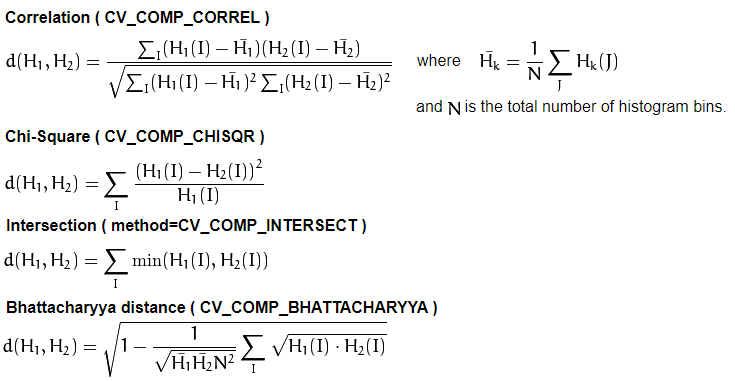
\includegraphics[width=\textwidth]{templateLaTeX-Eng/img/comparisonmetrics.png}
    \caption{\bf Histogram comparison methods described in [14]\footnotemark}
\end{figure}
\footnotetext{Source: \\
https://docs.opencv.org/2.4/doc/tutorials/imgproc/histograms/histogram\_comparison/histogram\_comparison.html}
Another image comparison method would be template matching. It basically finds areas in an image that match or are similar to a template image. The template, also called patch, has to be a rectangle. Since, in many cases, not all of the patch is relevant, masks can be created to isolate the parts of the template that should find the similarities. Essentially, the template is slid across the source and it is determined how well it matches each location. This results in metrics that can be compared and the highest value (or lowest, depending on the matching method) is chosen.
 
Another, and possibly the most efficient method, would be rotation invariant feature matching. Feature matching can most simply be described as taking features from one set and matching them with the features of another set by using some distance measure. The closest matching one is the one we are interested in.

As stated by Anders Hast and Andrea Marchetti in their paper about feature matching [15], feature points come in many forms. They can be Harris corners, difference of Gaussians or determinant of Hessian matrix.

 %=======================================================================================================  
 
 %=======================================================================================================  
 
\section{Information Retrieval}

The internet has seen an extremely high increase in users. Just as of April 2020, 4.6 billion people were registered as active internet users, which represents around 59\% of the global population [16]. Thus, the World Wide Web has become the go-to place for information. 
Chunmei Zheng, Guomei He and Zuojie Peng [17] have observed that due to the surplus of web servers, web pages and overall information present on the internet, users have to undergo an increasingly harder process in order to find whatever data they are seeking. This directly ties one of our concerns, the problem of finding reliable movie reviews conveniently and quickly.

As stated by the previously mentioned authors, web information retrieval has been a highly researched topic since the inception of the internet. Many methods have been formerly employed by a vast array of researchers. 

\subsection{Web Crawlers}

One of the simplest and most popular approaches is web scraping. Web scraping performs mass browsing and analysis of web pages. This process is automated by the construction of a web crawler, relieving the user from manual skimming through endless websites in order to find desired information.

Web crawlers, also known as "spiders", "ants" or "automatic indexers" and often simplified to "crawlers", are automatic systems that systematically parse the World Wide Web, in order to retrieve specific data. Said data is collected and given a form suitable for the user's purposes.

Given certain URLs, the crawler visits them and identifies all the elements it is concerned with. These elements are collected into the \textit{call frontier}, which are certain pages and data that need to be analyzed. By employing numerous recursive policies, the crawl frontier is visited, the corresponding websites are archived and the relevant information is stored.

Web scraping is a lot simpler than the classic web crawling used for indexing. Scraping systems make direct use of HTTP and is able to understand and parse all the elements used in HTML and other web development frameworks. Basically, the end goal of a web scraper is to fetch web pages, systematically parse its contents and extract the relevant data into a specialized form to make use of it in some other purpose.


\subsubsection{Beautiful Soup}
The China University of Geosciences scientists' approach to information retrieval was Beautiful Soup. Beautiful Soup is a Python library for analyzing HTML pages and extracting data. It works by parsing the given file and using idiomatic ways of navigating, searching and modifying the parse tree [18]. The library essentially turns the HTML file into a DOM tree and provides the user a number of operations for manipulating said tree. 

\begin{figure}[H]
    \begin{center}
        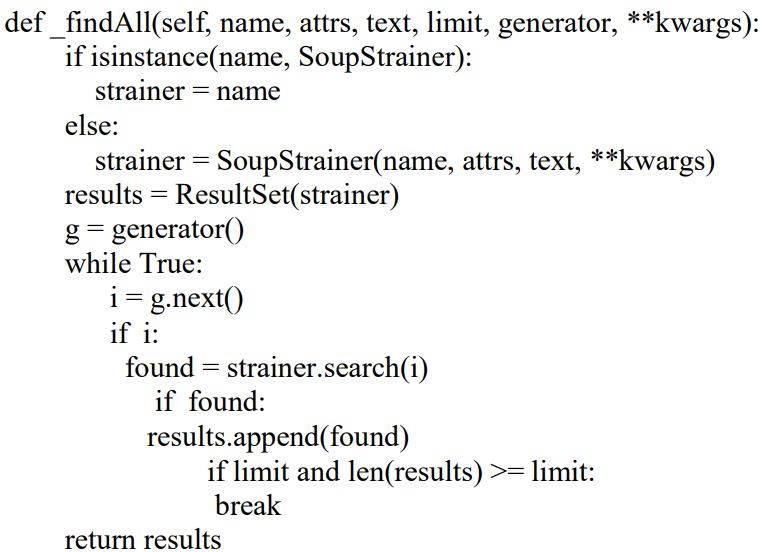
\includegraphics[width=300px]{templateLaTeX-Eng/img/findall.png}
        \caption{\bf Example of a \_findAll function from [17]}
    \end{center}
\end{figure}

\subsection{Machine Learning}

 Machine learning was an approach closely pursued by Sally Jo Cunningham, James Littin and Ian H. Witten [19]. They remarked that webpage data extraction and retrieval has many features that are fitting for artificial intelligence approaches. The authors suggested employing natural language text analysis in order to capture the nature of the webpages through which term vector models are built. These models are indexed, organized and ranked. The frequency of terms is analyzed and their importance is measured, taking rarity into account, each one being weighted by the number of appearances.
 
 The models extracted result in features from which certain classifiers can be extracted. Documents can then be compared and weighted by similarity metrics. Of course, many problems may arise in this process. Synonym and phrase identification has been a hot topic in this field.
 
 The last step of this process is creating a collection of therms that are indexed. In order to satisfy queries, the machine learning system may be required to parse through a number of collections. An algorithm that quantifies how much a web page matches the original query is employed and the highest-scoring one is returned.
 
 %=======================================================================================================  
 \newpage
 \section{The Android Operating System}
 
 Android is the most popular mobile platform, running on millions of devices world wide. In previous chapters, the sheer scale of the Android Operating System was discussed and it was determined as the best choice when it comes to mobile application projects. 
 
 The Android OS is mainly based on the Linux kernel and was originally designed for smartphones and tablets. As time went on, Android made it's way to other devices, such as smart watches, televisions, cars and internet of things devices, as well as many others. The fact that Google, the main developer and sponsor of Android, decided to make it a free and open source software, allowed for other companies to modify and enhance the source code in order to create their own custom operating system to be integrated into their devices. This allows for a more personalized experience that focuses on the needs of the company's users.
 
 The fact that Google made Android free and open source also encouraged developers with an interest in mobile applications to adopt it as their primary platform. Google understood the importance of aiding developers in achieving their goals and, to this day, the company provides continuous support. The Android Software Development Kit (SDK) is a set of resources, tools and frameworks designed specifically for Android. The SDK includes Android Studio, the integrated development environment (IDE) used to develop Android applications. Due to its popularity, Android developers have seen no shortage of online and offline resources to back them up.
 
 Android applications can be written in the Kotlin, Java and C++ languages, the former two being the most popular. In 2019, Google officially replaced Java as the preferred language for Android development with Kotlin. Despite this, Kotlin can still fully inter-operate with Java. 
 
 While the previously mentioned languages are used to implement the logic side of the Andorid application, the user interface is developed through XML files. XML stands for Extensible Markup Language and is a markup language, similar to HTML, used define and link graphical elements. There are many advantages to XML, like its simplicity and scalability, but the main one is the fact that Android knows how to display data consistently, regardless of the host device. Thus, most of the time, the developer won't have to be concerned with the sheer variety of screen shapes and sizes distorting the way their UI is displayed.
 
 The Android Operating System started with a public release as a beta on 2007. The first official version of the OS was Android 1.0, released on 2008. Since then, Google continuously developed and enhanced the operating system, delivering uninterrupted updates since its inception. The latest version of is Android 11 Beta, but the latest stable and commercially available one is Android 10, released on 2019. 
 
 \newpage
 \subsection{Android Architecture}
 The way a project is structured may be one of the most important attributes of any application. A good architecture provides scalability and maintainability. As the pioneer of clean code, Rober C. Martin, or as most would know him "Uncle Bob", claims that following certain software architecture rules can dramatically boost productivity and lifespan of any software system [20]. As he says, even bad code can do its job. But the cleanliness of the code is what makes or brakes the app on the long term. Thus, the backbone of any application is its architecture.
 
 While not exclusive to Android, there are three main architectural patterns that define Android development: MVC, MVC and MVVM. The problem lies in choosing one of them.
 
 Author T. Lou has done extensive research comparing the three patterns in his master thesis paper [21]. He concluded that MVP and MVVM are better than MVC in terms of performance, testability and modifiability. The former two successfully provide high cohesion and low coupling to Android applications. 
 
 Google doesn't impose any one architectural style for mobile app development. For some time, MVP was the most used pattern. This has recently changed. In 2018, Google introduced Android Jetpack. Android Jetpack contains a collection of Android libraries that encapsulate all the best practices. Since all the libraries are independent of each other, they are frequently updated and well documented. One of the most important features of Jetpack is their architecture-related components which favor the MVVM architectural pattern.
 
 There are some clear advantages MVVM has over MVP:
 \begin{itemize}
     \item Better separation of responsibilities which leads to low coupling. 
     \item The low coupling, in turn, leads to easier testing.
     \item Code reuse. The ViewModel code especially is highly reusable.
     \item Higher maintainability which is suitable for agile work methodologies.
     \item High compatibility with other design patterns, such as Command, Factory, Singleton, etc.
 \end{itemize}
 
 \subsection{Activity vs Fragment}
 Activities are the primary components of an Android application. They are single, standalone modules that correspond directly to a single UI screen and its functionality [22]. Activities can be personalized as the developer wants by adding visual elements, such as buttons, text, images and many more. The visual part of an activity is designed and developed inside XML files. However, having one XML file for each activity is only one of the options available.
 
 As stated by Neil Smith in his Android development book [22], the better alternative is to break the activity into different sections. These sections is what are called Fragments. While very similar to activities, fragments provide better lifecycle management and reusability, are more lightweight and come with more development tools. The introduction of Android Jetpack practically solidified this approach as the winner in the "Single activity - multiple fragments vs multiple activities" debate.
 
 \subsubsection{Lifecycles}
 
As the user navigates through an Android application, hopping from screen to screen, opening and dismissing dialogs and coming back to previous screens, Activity and Fragment instances transition through a number of states in their lifecycle. Each lifecycle state has its own callback method, which can be configured as the developer wants. 

\begin{figure}[H]
    \begin{center}
        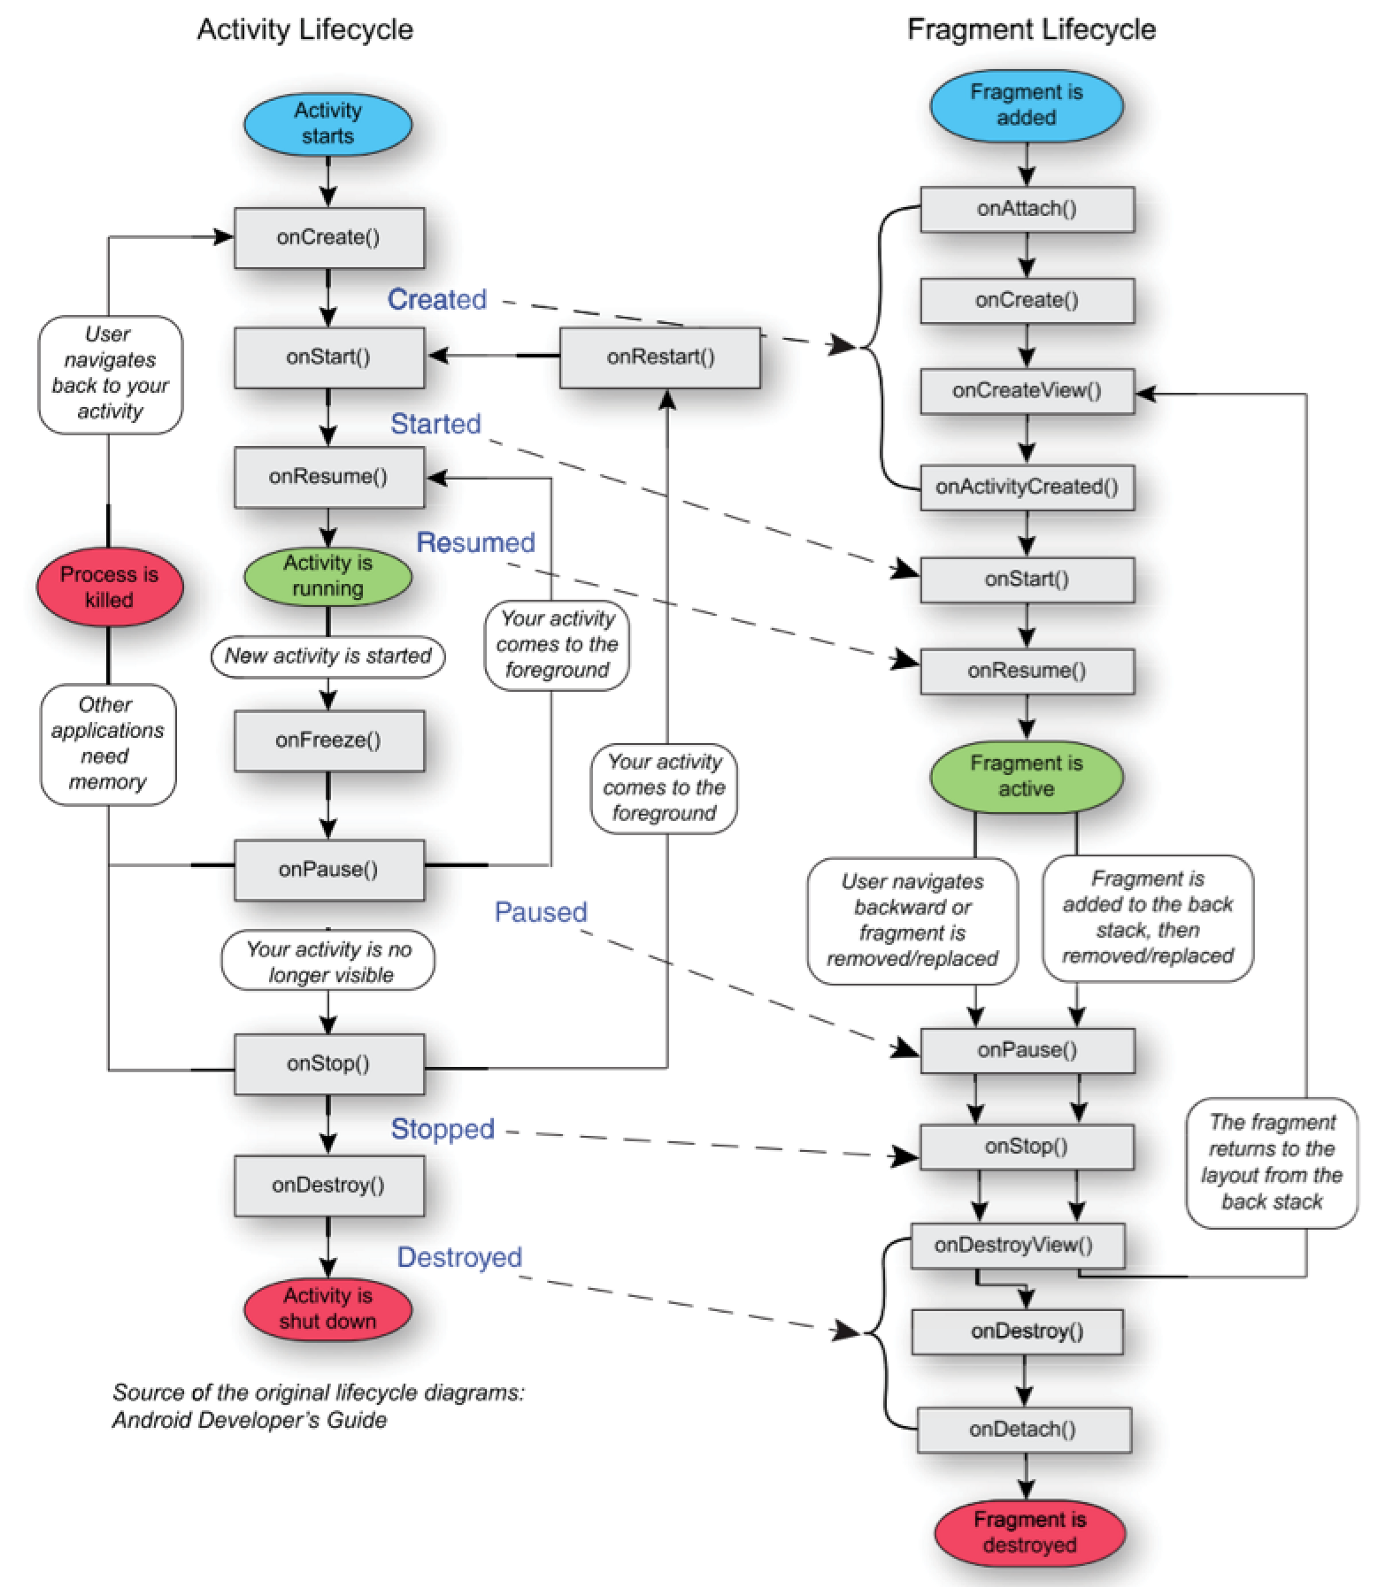
\includegraphics[width=300px]{templateLaTeX-Eng/img/lifecycle.png}
        \caption{\bf Comparison between the Activity and Fragment lifecycles\footnotemark}
    \end{center}
\end{figure}

 \footnotetext{\textit{Source: https://medium.com/@elye.project/activities-or-fragments-a-little-sharing-c1ddc1041f79}}
 
 Properly handling and using lifecycles is very important in the development process of an application. This is why, Android Jetpack provides so-called Lifecycle-Aware components. These components perform operations in response to a change from a state to another in the lifecycle of an activity or fragment. With their help, better code can be achieved. The lifecycle-aware components also make the application organized better, more lightweight and easier to maintain, while also preventing memory leaks and race conditions. 
 
%=======================================================================================================  

 \chapter{Analysis and Theoretical Foundation}

%=======================================================================================================  
\vspace{1cm}
\section{Proposed Solution}

The purpose of my thesis is to design and develop a system that allows users to search for any desired movie and see relevant reviews of the movie that come from numerous sources. The project aims at decreasing the time a user would need to make a decision on what movie to watch based on its reviews. The system will also allow for searching movies by taking a photo of its poster. 

The main goals of the system are:
\begin{enumerate}
    \item Implement a poster recognition software that receives an image containing a poster and returns the title of the poster.
    \item Create a web crawler that retrieves movie reviews.
    \item Design and develop an Android mobile application that encapsulates the functionalities mentioned above.
    \item Since the first two goals should be able to work as standalones, we need to find a way to expose their functionality so that they can be used in the third goal. This will come in the form of an API.
\end{enumerate}

So the proposed system would essentially be an Android application that calls endpoints of an API whose functionalities include poster image searching and movie review retrieval. 

%=======================================================================================================  

%=======================================================================================================  
\newpage
\section{OpenCV and Python}
As stated in chapter 3, OpenCV is an open source library that is used for image and video manipulation and analysis. Being open source, it opened itself to many improvements from the community and made itself the most popular library of its kind. That being said, it's no wonder the sheer amount of resources, tutorials and overall support available for developers who opt to use OpenCV. Thus, choosing OpenCV as the primary library that will be used for  the poster recognition phase of my project is a no-brainer.

OpenCV is written in C++ and its main interface is in C++. Even so, bindings exist so that it can be used in Python and Java, or even MATLAB. The library doesn't impose any one language on the developer, which is another benefit it provides. 

When choosing a language for image processing software development, one's first instinct would be to choose the one with better performance. From that standpoint, C++ clearly has the edge over the others. C++ compiles directly to machine code which ties it more closely to the CPU. This results in faster execution and more time efficient programs. C++ also favors using existing memory. Which in turn makes it more memory efficient as well. 

Having said that, C++ does have its disadvantages. C++ is infamously harder to learn and write. It is strongly-typed and leaves very little margin for error. This means, the development phase of a software is much more cumbersome when using C++. This is where Python comes in. While notably slower than C++, Python was designed to be as simple as possible. It is one of the easiest languages to learn and code. The fact that it requires an interpreter is what gives it slowness but that may not be such a bad thing. Python-OpenCV is essentially a wrapper over the original C++ implementation. This makes the performance factor less impactful. Basically, you get the best of both worlds, the performance of C++ along with the simplicity of Python.

Python's popularity is nothing short of impressive. Claiming the top spot in the popularity chart with a share of over 31\%, one would only have to look at the incredible vast application the language is used for. Among the many uses it has, most notably we can mention: embedded applications, data science and visualization, CAD applications, embedded applications game development, web development, web scraping and audio/video applications. The latter two are the ones we're most interested in.

%=======================================================================================================  

%=======================================================================================================  
\section{Edge Detection}
The first major step in our poster recognition system is to identify the poster itself. A user submitted image can have a lot of extra data that is not needed. Also, the image almost certainly won't be 100\% perpendicular to the poster so some perspective skewing is to be expected.

We can assume that any poster a user would photograph has a rectangular shape and has the standard size ratio of 2:3, or close to it. Thus, the problem reduces to finding all rectangular shaped objects in the image and choosing the one that is most likely the poster.

Canny edge detection is one of, if not the most popular edge detection algorithm. Developed by John F. Canny, it is a multi-step algorithm that detects pixels in images at which the level of brightness changes abruptly. Those pixels can be called edge points.

For the canny image to be applied correctly and efficiently, a few preprocessing operations must be performed.

\subsection{Preprocessing Steps}
Preprocessing operations process input data into output that is to be used as input in some other operation or process.

\subsubsection{Grayscale Conversion}
Grayscale images are images whose pixels only have one representative value. That value can be viewed as the amount of light the pixel has, carrying only intensity information. Thus, grayscale images are images that only contain shades of gray, having as minimal and maximal values black and white respectively.

The actual conversion from a color image to a grayscale image is straight-forward. It works by taking each pixel and averaging the values of the red (R), green (G) and blue (B) and assigning the resulted value to the pixel. Though simple, this method can bring up some problems. 

Since not all three channels have the same contribution to building a pixel, the equal part assignment to the computing of the average may not be fair. This is why a weighted average method was composed. Due to the difference in wavelength, each component has to be given a proper weight at averaging. The equation of (0.3 * R) + (0.59 * G) + (0.11 * B) is one of the popular ones.

\subsubsection{Thresholding}
Binary images are grayscale images whose pixels exclusively have values of either 0 or 255. Thresholding is the process of creating a binary image by replacing its pixel values with 0 if they have an original value lower than the threshold value, or 255 if they have an original value higher than the threshold value.

\subsubsection{Morphological Operations}
Morphological operations are simple transformations to the shapes of an images. They are ususally performed on binary images. 

Erosion is the operation that "deletes" all external pixels from an image. This means that if, in a binary image, all white pixels are objects and all black pixels are the background, erosion will transform all boundary points of objects to black. This is used to remove noise and small objects that wouldn't matter in the big picture. Essentially, any white pixel that has a neighboring black pixel is turned to black.

Dilation is the opposite operation of erosion. This operation is used to add an extra layer of pixels to all objects. Thus, any black pixel that has a neighboring white pixel is turned to white.

The next two operations are different combinations of the first two. Opening is a morphological operation that is composed of an erosion followed by a dilation. This is used for removing small objects while bigger object suffer little to no change. Closing is the opposite operation of opening. It is composed of a dilation followed by an erosion. It is mostly used for filling holes while not modifying the overall object sizes and shapes.

The reason morphological operations need to be used before performing the Canny Edge Detection algorithm, is to remove any irrelevant objects or imperfections that may result after performing the thresholding operation. Of course, which morphological transformations need to be performed and in which order is very important. This will have to be studied further in the implementation phase so that many combinations can be tested on an input image directly.

\begin{figure}[H]
    \begin{center}
        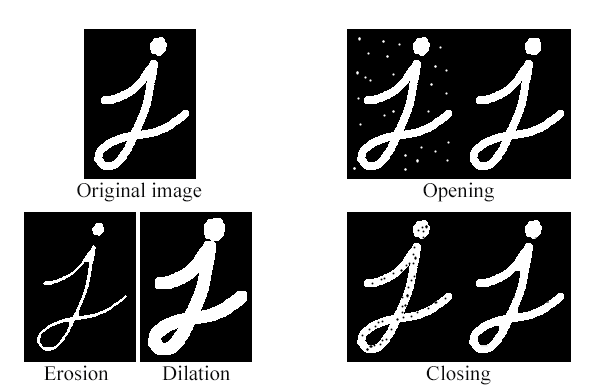
\includegraphics[width=400px]{templateLaTeX-Eng/img/morphologicaloperation.png}
        \caption{\bf Examples of morphological operations\footnotemark}
    \end{center}
\end{figure}
\footnotetext{Source: https://docs.opencv.org/trunk/d9/d61/tutorial\_py\_morphological\_ops.html}

\subsection{Canny Edge Detection}
The Canny Edge Detection algorithm is comprised of 4 main steps:
\begin{enumerate}
    \item Minimise the noise so that there are as little falsely detected edge points. False edges can severely affect the edge detection so false edges must be detected and removed as much as possible. The noise reduction process will be performed with a Gaussian blur. A technique called image convolution along with a 5x5 Gaussian kernel. 
    \item After the original image is smoothened in the previous step, the image gradient has to be computed. The gradient of a point is a vector with the direction of the intensity variation around that point. The computation of the gradient can be mathematically defined as a continuous function constructed by partial derivatives in the x and y coordinates, like so:
    \begin{figure}[H]
        \begin{center}
            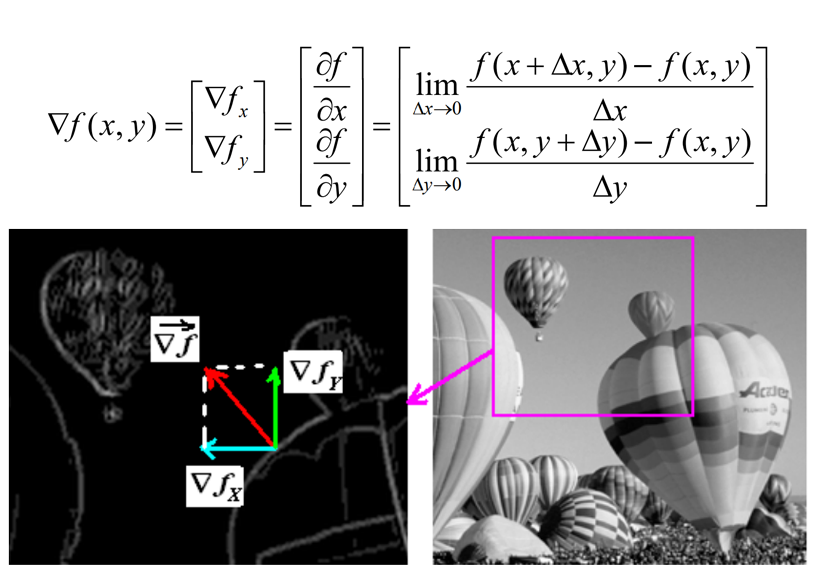
\includegraphics[width=350px]{templateLaTeX-Eng/img/imagegradient.png}
            \caption{\bf Image gradient computation\footnotemark}
        \end{center}
    \end{figure}
    \footnotetext{Source: http://users.utcluj.ro/\~igiosan/Resources/PI/L11/PI-L11e.pdf}
    In the case of digital images, the gradient can be approximated using convolution with Prewitt, Sobel or Robert/Cross kernels. 
    The direction of the gradient is always perpendicular to the edges, being rounded to the four agles that represent the vertical, horizontal and the two diagonal directions.
    \item Even after the image gradient is computed, several non-edge points can still exist. In order to filter the true edge points, a process called non-maxima suppression has to be performed. It's purpose is to thin out the encountered edges by only keeping the edge pixels with that are local maximums in their neighborhoods in the direction of the gradient. This step will result in the edges having a thickness of exactly one pixel.
    \item The last step is called Hysteresis Thresholding. It is concerned with differentiating true edges from false edges, and dismissing false edges. This is done with a form of thresholding in which any edges smaller than the maximum threshold value and bigger than the minimum threshold value are considered as true edges. Before finally classifying those edges as the final true edges, their connectivity has to be analyzed. 
\end{enumerate}

\begin{figure}[H]
    \begin{center}
        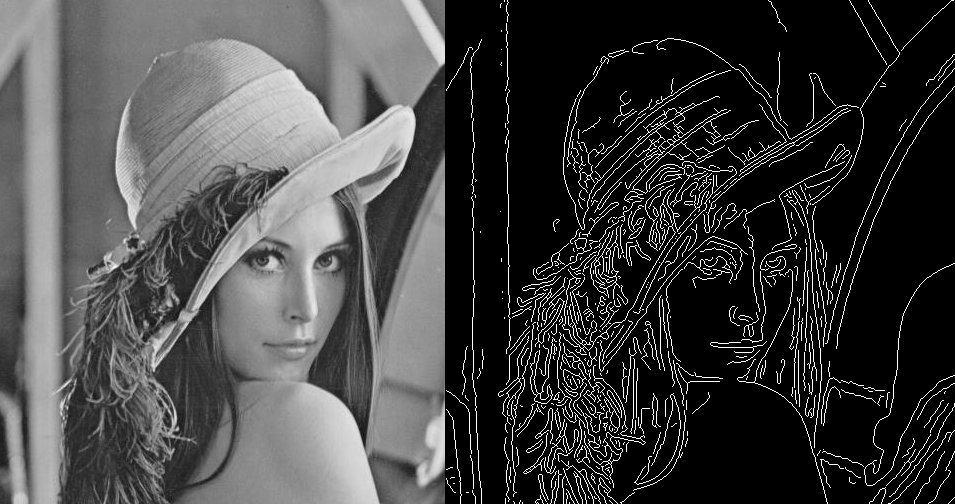
\includegraphics[width=400px]{templateLaTeX-Eng/img/lanacanny.png}
        \caption{\bf Canny Edge Detection performed on Lenna}
    \end{center}
\end{figure}

Now that all the edges are computed, they can be analyzed and information about their shape, size and overall position can be extracted.

The OpenCV Python library provides implementations for all the operations talked about in this section. Some of the fucntions the library provides are: cv.CvtColor, cv.GaussianBlur, cv.Threshold, cv.morphologyEx, cv.Canny.

%=======================================================================================================  

%=======================================================================================================  
\newpage
\section{Contour Features}
Having extracted the contours, the next step is to interpret them. Though we have all the necessary edges, we also have unnecessary ones which must be dismissed. Firstly, we have to extract each individual contour as an array of points. That way contours can be examined independently. This can be done by any labeling algorithm

The next step is to parse the collection of edges and find those edges that have the properties we are looking for in a poster:
\begin{itemize}
    \item Closed perimeter contour.
    \item Four sharp corners.
    \item Aspect ratio of roughly 2:3.
\end{itemize}

To make things easier, all the contours with a small perimeter can be dismissed as the poster is assumed to be the central object in the photo taken by the user.

The first two features can be checked for in the context of a simple border tracing algorithm. The basic functionality of such algorithms consists of parsing all the pixels that are connected in a clockwise or counter-clockwise manner.

In order to check for the first property, one can parse all the pixels of a contour in order and marking each pixel as visited at each step. When arriving at the end, if all the pixels of the contour are marked as visited and the last one neighbors the first pixel, it means that the contour has a closed perimeter and the can be checked for the other features.

For the second feature, when going from one pixel to the next, a direction can be extracted. When choosing the next pixel, the 3x3 neighborhood of the current pixel is analyzed. Depending on what position the next pixel resides in, a direction can be extracted based on the following figure:

\begin{figure}[H]
    \begin{center}
        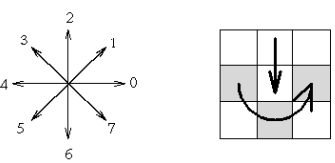
\includegraphics[width=200px]{templateLaTeX-Eng/img/borderdir.png}
        \caption{\bf 8-Connectivity direction notation and pixel neighborhood sequence for counter clockwise tracing\footnotemark}
    \end{center}
\end{figure}
\footnotetext{Source: http://users.utcluj.ro/\~igiosan/Resources/PI/L6/PI-L6e.pdf}

By storing the direction of the current and previous picture, corners can be detected. For example, if the previous direction was 1 and the current direction is 6, we can assume that the current pixel is a corner that unites a 45 degree slope edge with a perpendicular edge. 

After this operation we should be left with an array of corners. If the array contains 4 elements we can assume that the edge represents a rectangle. Having the four points, one can simply calculate the length of the two defining edges of the rectangle and check if it has a ratio close to 2:3.
%=======================================================================================================  

%=======================================================================================================  
\section{Color Spaces}
The user submitted images will be represented in the RGB color space. A RGB color can be thought of a color that can be constructed by adding together different variations of the red, green and blue colors. This color model is used for representing and displaying images on screens, such as computer screens and televisions. The sheer simplicity of having three values, ranging from 0 to 255 to represent a color is what makes it so easy to process from a mathematical standpoint.

That being said, there is one alternative that is considered better when processing digial images. The HSV color space is how researchers defined as being more similar to the way the human eye perceives colors. HSV stands for Hue, Saturation, Value. In this color space, colors are represented by their hue, which defines the actual color type (i.e. red, blue, etc.), saturation, which represents the intensity or purity of the color and the value, also known as brightness.

Extensive research has shown that the HSV color space is better for image processing applications. This is because it is much better at picking up on details and subtleties that result from lighting, noise and other environmental factors.
\vspace{1cm}
\begin{figure}[H]
    \begin{center}
        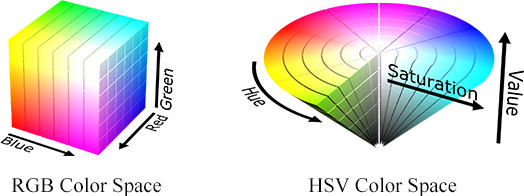
\includegraphics[width=350px]{templateLaTeX-Eng/img/rgbhsv.png}
        \caption{\bf Comparison between the graphical representations of RGB and HSV}
    \end{center}
\end{figure}
%=======================================================================================================  

%=======================================================================================================  
\section{Histograms}
Histograms represent the distribution of pixel values across an image. They are graphically represented as a bar graph where the horizontal axis represents the tonal variations of the pixels and the vertical axis represents the total number of pixels for each tone.

The main purpose of histograms is to view the tonal distribution of digital images. They convey very useful information for photographers and image editors, capturing lost detail that wouldn't be observed at a glance. Image processing systems have also benefited a lot from histograms, many algorithms making use of them for dynamic brightness and contrast manipulation. In computer vision, the shape of the histograms is also analyzed, by making use of the "peaks" and "valleys". This leads to many thresholding applications which, in turn, are used in a myriad of other complex algorithms. 

In our case, image histograms will be used in the comparison of two posters. Since a histogram represents the tonal distribution of an image, if two posters have similar histograms, there is a higher chance that the posters are the same. 
%=======================================================================================================  

%=======================================================================================================  
\section{Web Scraping with Python}
As stated in previous chapters, web scraping is the process of analyzing, extracting and structuring specific data from HTML/XML content. Our project is concerned with fetching movie review information from numerous sources/websites, in order to provide a place where all reviews of a movie are aggregated for viewing. This will aid the user in reading all the most relevant reviews of a movie and removing the needlessly cumbersome task of navigating through a myriad of websites. Usually, websites provide APIs that allow anyone to access their data. However, there are many cases in which the APIs are incomplete or lack proper documentation, making them virtually unusable. This is where web scraping comes in. In this regard, Python provides a series of modules that can be used to automate the fetching of HTML content directly from the web.

Beautiful Soup is a very popular Python library used for scraping information from the web. It is usually used in concordance with the Requests module, which is used for sending HTTP requests. 

\subsection{Requests}
HTTP, which is short for Hypertext Transfer Protocol, is the main way of exchanging information over the internet. Everyone uses HTTP requests when surfing the web, even if they are aware of it or not. Browsers send HTTP requests for retrieving HTML pages and other content associated with them. When a HTTP request is sent, the receiver of that request, the web server, handle them by retrieving the needed data and returning response messages that incorporate said data.

\noindent An overview of the steps taken when performing a HTTP request:
\begin{itemize}
    \item The client sends ah HTTP request to the web.
    \item The corresponding web server receives the HTTP request.
    \item The web server processes the request.
    \item The web server returns an HTTP response containing the successfulness of the request accomplishment.
    \item The client/sender receives the response and interprets its contents.
\end{itemize}

The Requests library is one of the most popular Python library out there. Its most common usages are to perform GET requests to APIs and to retrieve raw HTML content. The only resource the Requests library needs in order to fulfill a request is an URL. The two important components of the URL that need to be specified are: 
\begin{enumerate}
    \item The Protocol Identifier: \textit{http:, https:, ...;}
    \item The Resource Name: \textit{domain/path};
\end{enumerate}

The simplest usage of the Requests library would look like this:
\begin{figure}[H]
    \begin{center}
        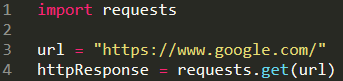
\includegraphics[width=200px]{templateLaTeX-Eng/img/requestsexample.png}
        \caption{\bf GET request to www.google.com using the "requests" module}
    \end{center}
\end{figure}

\subsection{Beautiful Soup}
Beautiful Soup is the popular Python module used for extracting data from HTML and XML files. Due to it's simplicity, it is best used for small-scale systems.

Some knowledge is required from the programmer in order for Beautiful Soup to be used to its full efficiency. The first one would be basic HTTP understanding which was discussed in the previous chapter. The second requirement is basic HTML and CSS knowledge. The HTML markul language basically shapes the way all the elements are formatted and fitted inside a web page. CSS instructions provide the rudimentary HTML elements with numerous styles and decorations.

Tags are the defining elements of the HTML language. Tags are keywords enclosed in diamond brackets which define how HTML files are supposed to be displayed. HTML tags can be enclosed within other other HTML tags. Doing this repeatedly is will result in a HTML hierarchy. This is where Beautiful Soup operates.

The most important part of using Beautiful Soup is the inspection of the web page to scrape. The overall structure and hierarchy must be closely analyzed. The easiest way to do so is to use any browser's developer tools. When web scraping, one can easily spend more time in the browser than in the code editor with the actual programming. This is why an intense knowledge of the browser's developer tools and how to leverage them must be an important skill in every web-related programmer's arsenal. The main developer tool used in web scraping is the element inspection tool. The inspection tool allows users to click any visual element in the web page and see the HTML, CSS and Javascript code that went into creating and rendering it. Of course, the entire HTML hierarchy tree can also be viewed and parsed accordingly. 

The steps for using Beautiful Soup to scrape any website are the following:
\begin{enumerate}
    \item Perform a HTTP request using the "requests" Python module and providing a valid URL.
    \item Receive the HTML content as the response.
    \item Examine the HTML structure and identify which elements we are concerned with and what data needs to be extracted.
    \item Pass the HTML content to Beautiful Soup for processing.
    \item Use Beautiful Soup to find certain elements of interest and extract their data.
    \item Process the extracted data and output it in the desired format.
\end{enumerate}

Here's a simple example of retrieving the width in pixels of the Google logo present in Google's homepage: 

\begin{figure}[H]
    \begin{center}
        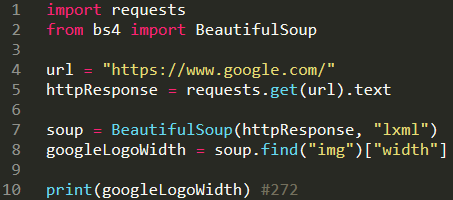
\includegraphics[width=300px]{templateLaTeX-Eng/img/bs4example.png}
        \caption{\bf Retrieving Google's logo width using Beautiful Soup}
    \end{center}
\end{figure}

Beautiful Soup's popularity is not surprising when taking into account it's simplicity and how well it performs. It can be said that it is the best web scraping library for building small scale web crawlers quickly and efficiently.
%=======================================================================================================  

%=======================================================================================================  
\section{Communication Between Systems}
We stated in numerous of the previous sections that we need a way to make all the components in our system communicate easily. Nowadays, almost all devices we commonly use have access to the internet. Smartphones, laptops, PCs, smartwatches and even home appliances communicate with each other and with other systems through the internet. Another statement that has been thrown around in this paper is that HTTP is one of the best "bridges" for exchanging information on the web. By that logic, we need to make our components interact throught the power of HTTP requests.

\subsection{Application Programming Interfaces}
Application Programming Interfaces, or API for short, are pieces of software that makes interactivity between systems possible. In simple terms, it is a messenger that receives requests from a sender and, based on the request, it tells another system what to do. Afterwards, the API delivers the result back to the sender.

Application Programming Interfaces simplify systems by hiding its underlying implementation and only exposing certain operations, attributes or objects. While there are many types of APIs, the one we're most interested in is the Web API. Also called a web server, it is an interface that consists of numerous endpoints corresponding to specific actions or objects, which are accessed by means of the HTTP protocol. 

\subsection{REST}
REST stands for Representational State Transfer and is an architectural style first introduced in 2000. Roy Fielding, the creator of REST, developed REST as a way to describe the larger architecture concepts behind how the web is supposed to work. He created REST as an architectural style intended for long-lived network-based applications. Basically, REST is a standard on how computers should communicate with each other. Systems that comply with REST are called RESTful systems. There are two major attributes that characterize REST.

The implementation of the client and the one of the server can be done independently of each other, when using the REST architectural style. This is very important as changes in one system won't affect the other systems. This low coupling is what attracts most developers to rest. Additionally, high cohesion is achieved because of the modular nature of RESTful systems. There is a clear separation of concerns, each system performing its own separate tasks.

The second characteristic that REST has is statelesness. Systems that follow the REST architectural style are stateless, meaning that the client doesn't know the server's state and the server doesn't know about the client's. They simply communicate through message and only know about the message's existence. No session is initiated between the client and the server and no states or message history is kept by any party involved. HTTP requests are isolated and independent of each other. The responsibility of providing the necessary data in order to make the communication successful is held by both parties. 

There are many advantages to using REST:
\begin{itemize}
    \item Provides support for various types of data, such as JSON, XML, text, etc.
    \item Has better support for browsers than other communication protocols.
    \item Great performance.
    \item Low bandwidth usage.
    \item It is easy to modify because components are isolated.
    \item Scalability. Maybe its most important feature, it is the reason REST was originally adopted. 
\end{itemize}

\subsection{Django}
 Now that we've established that our mobile application will be interacting with our other components through the use of a RESTful API, it's time to choose a framework that is suitable to our needs.
 
 Since we use Python for our poster recognition software and also for our web scraping system, it would be great for our API to understand and run Python code. There are many languages with suitable frameworks for building RESTful APIs. Java has the Spring Framework, Javascript has Node.js. Both of those, also have modules that allow to build and run Python/.py, scripts. Even so, the performance is severely hindered an in our day and age, users will boycott an application if it delivers results too slowly. Thus, in order to bypass the usage of extra components that interpret Python code, a better solution would be to build the API directly with Python.
 
 Django is a high-level Python-based web framework that allows the creation of websites. It also provides a flexible and powerful tookit for building Web APIs. The versatility of Django is what attracts most developers to use it. One can build any type of web application that works on any kind of system. With numerous templates and database building alternatives, it's not hard to see where it's popularity came from.
 
 As stated before, Django is written in Python. This is one of the features that attracts most developers. Capable of running on almost all platforms, the fact that it doesn't tie itself to any single one greatly increases it's portability. This, in turn, means that hosting Django applications is easier as it does not need a specific infrastructure. 
 
 Django developers take pride in the fact that the framework contains everything needed to achieve what any other developer needs. All the components needed to build a web application are provided by Django and all of the work seamlessly together, following well defined design principles. The documentation is extensive and kept up to date.
 
 The Python framework also helps developers by providing numerous security mechanisms that are automatically incorporated. Django takes care of the many vulnerabilities that might arise during development of complex systems. 
 
 Django defines it's own architectural pattern of Model View Template, or MVT. Similar to Model View Controller, MVT provides a low-coupling, high-cohesion architecture that separates components into modules that handle different operations:
 \begin{itemize}
     \item URLs: The URL mapper redirects HTTP requests to the corresponding view. The URL mapper can also preprocess the data passed through the request.
     \item View: Receives requests and return HTTP responses. Views can access any needed data or algorithms needed to satisfy the HTTP requests via the models.
     \item Model: Python objects that define the data of the application and its structure. It also provides operations to manipulate said data.
     \item Template: Text files that define the layout of files. They can dynamically create HTML pages through HTML templates and populate them via the models. They are not exclusively used for HTML files.
 \end{itemize}
 
 \begin{figure}[H]
    \begin{center}
        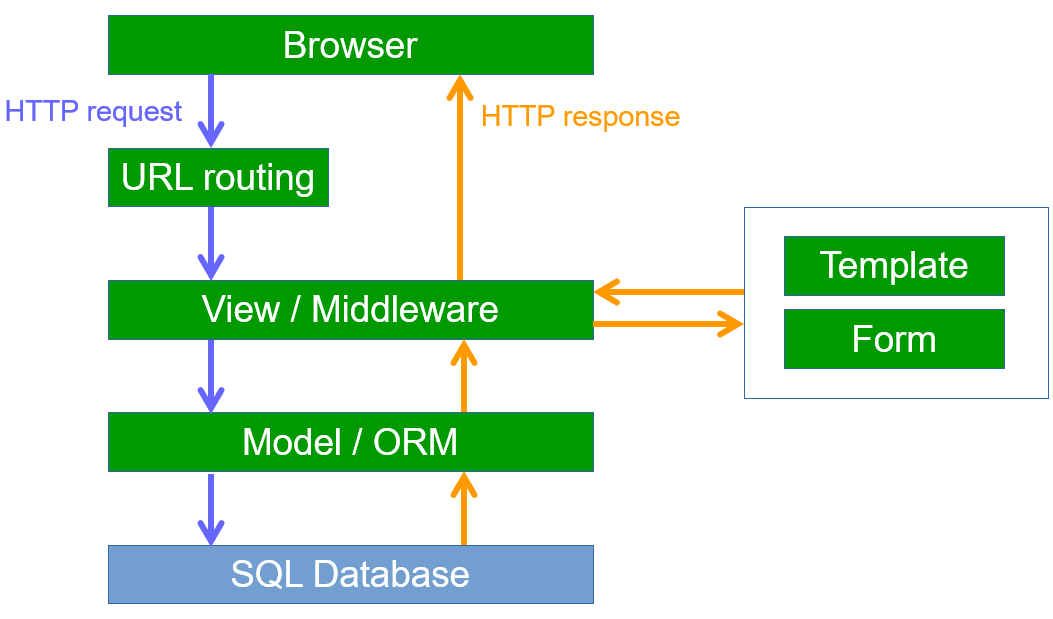
\includegraphics[width=400px]{templateLaTeX-Eng/img/djangoarch.png}
        \caption{\bf Django's architecture\footnotemark}
    \end{center}
\end{figure}
\footnotetext{Source: https://fleschenberg.net/django-architecture-diagram/}
%=======================================================================================================  

%=======================================================================================================  
\section{Android Jetpack}
Android Jetpack is a set of libraries introduced by Google in 2018. The purpose of those libraries is to provide developers an easy way to follow best practices, write as little boilerplate code as possible and build consistent and state-of-the-art Android applications. Using Android Jetpack, developers won't need to worry about backwards compatibility and other tedious tasks that represented a problem in the past.

Jetpack libraries can be used alone or in unison with each other. Each of them provide a specific solution to a specific problem that developers face in the development process of a mobile application. I will present the two most important components I intend to use in my project.

\subsection{Navigation}
The Navigation component of Android Jetpack handles the user's app journey. The user-app journey refers to all the interactions a user has with the application that result in navigating from screen to screen. Whereas navigating was a very daunting task before Jetpack, the new navigation component removes all the complexity and ensures consistency and a predictable UX by following a set of principles. The Navigation component consists of three main parts:

The Navigation graph is an XML resource that defines the destinations and the actions and transactions between them. It takes the form of a graph in which the nodes are the screens of the application and the edges are the paths a user can take.

The NavHost is the empty container in which destinations are swapped in and out. It is usually hosted inside an activity and displays fragment destinations defined by XML layout files.

The NavController is an object that is concerned with managing the app navigation within the NavHostFragment. It is the component that actually oversees which destination is currently displayed and which destinations are the next to be displayed. It tells the NavHost the appropriate destination to display.

\subsection{Data Binding}
Data binding is the technique of binding data or information sources to consumers and synchronizes them. This means that any change in the source data will reflect on the consumer end as well. This goes vice versa. 

The Databinding component introduced by Android Jetpack is one of the most popular ones. It is a support module that allows the binding of UI components displayed on the screen to data sources. The library helps users minimize the application logic code to link and update user interface elements.

\subsection{Lifecycle}
These Lifecycle library provides a myriad of lifecycle-aware components. These components perform actions in response to lifecycle state changes in the context of activities or fragments. The lifecycle-aware components help developers achieve better organization, less complex and unnecessary code and an easier maintenance process. Since managing lifecycles poorly can lead to memory leaks and race conditions, the Lifecycle library makes applications less error-prone.
%=======================================================================================================  

%=======================================================================================================  
\chapter{Detailed Design and Implementation}

The purpose of this chapter is to present all the design and implementation details of the thesis project. A general overview of the project will be describes, after which architectural and development details will be laid out. This chapter will also present every component that is part of the overall system, what purpose they serve and how they fit in the system.

%=======================================================================================================  
\section{General Overview}
The two main themes of this project are time efficiency and convenience. It will help its users search for movies they want to watch and read a conglomerate of reviews for those movies. The project aims to provide a faster and easier decision making process and will help users get a rough estimate of whether a movie satisfies his/her needs by making all the information available in one place. From the user's perspective, the system will take the form of an application that can be accessed as easily as possible, literally within reach of anyone.

The project will take advantage of a device most of the population has access to at any time of the day, the smartphone. Taking the form of an Android application, my thesis project will be able to find any movie, retrieve and display details about it, scour the web for the most relevant reviews and provide useful and relevant recommendations based on its user.

One of the goals of this project is for it to be as modular as possible. This will lead to low coupling and high cohesion, two of the most important design principles every developer should take into consideration. The project will be broken down into a series of components, each one having its own purpose and being as independent as possible. This leads to a very easy maintenance phase, as well as the opportunity of further scaling and adding improvements as time goes by. The modular characteristic of the project also leads to easier testing. As each component is independent, they can be tested as standalones. No hidden dependencies have to be taken into account.

In order for the application to work as intended, we aim to follow the best, state-of-the-art practices. The behavior of the project must be predictable, the user experience must be as smooth as possible. We aim to use all the latest and most stable versions of the technologies available in order to achieve this.

\section{Use Cases}
As a movie review aggregation application, our project won't many functionalities from the user's point of view. The application must be easy to use, it's functionalities must stand out to the users and must be as unambiguous as possible. User interaction should be as smooth as possible, the amount of taps one should make to reach a desired page should be minimal. The main functionalities the user is concerned with are the following ones:
\begin{itemize}
    \item Authenticate into the application.
    \item Search for a movie (either manually or through image search).
    \item View a movie's details.
    \item Read a movie's reviews.
    \item Browse through movie recommendations.
\end{itemize}

 \begin{figure}[H]
    \begin{center}
        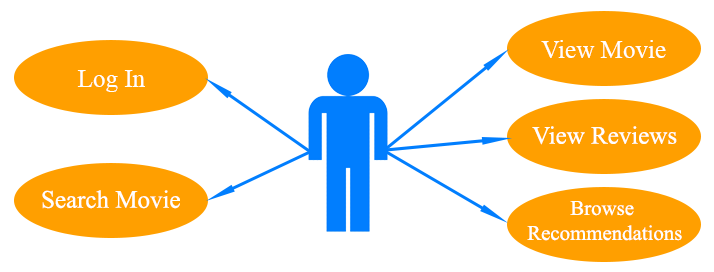
\includegraphics[width=400px]{templateLaTeX-Eng/img/UseCaseDiagram.png}
        \caption{\bf Use case diagram\footnotemark}
    \end{center}
\end{figure}
\footnotetext{This may not be a complete list of all the functionalities the application has.}

\section{Flow of Events}
 \begin{figure}[H]
    \begin{center}
        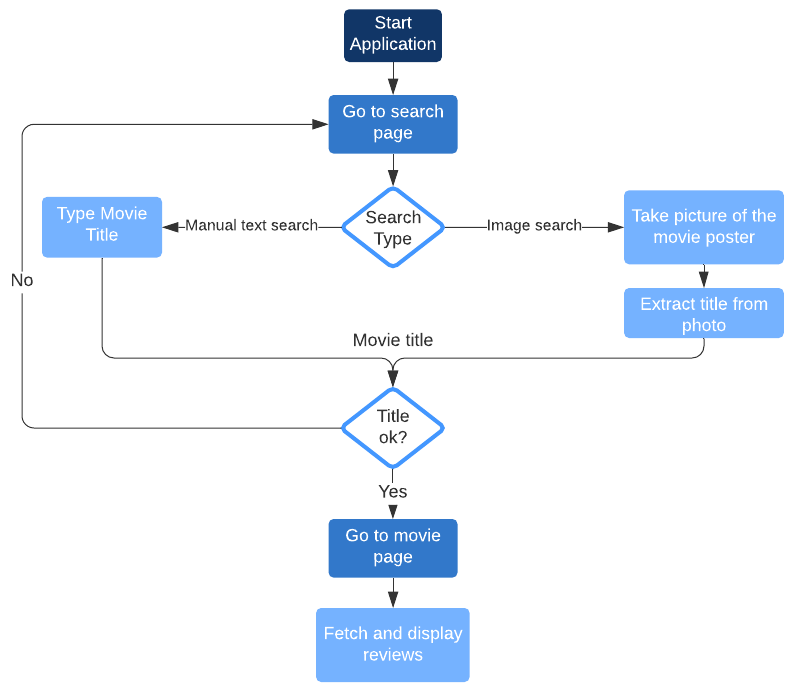
\includegraphics{templateLaTeX-Eng/img/flowchart.png}
        \caption{\bf Basic flow of the main application use case.}
    \end{center}
\end{figure}
This is the main flow of events the application and user follows in order to find reviews of a particular movie. The use case starts when the application is opened by the user for the purpose of reading a certain movie's reviews. Steps:
\begin{enumerate}
\itemsep0em
    \item The actor navigates to the application’s search page.
    \item The application displays the search alternatives:
    \begin{enumerate}
        \item The user types the title of the movie.
        \item The user takes a photo of the movie's poster.
        \begin{enumerate}
            \item The application extracts the title from the photo.
        \end{enumerate}
    \end{enumerate}
    \item The application validates the title.
    \item The user navigates to the movie page.
    \item The application fetches and displays the reviews of the movie.
\end{enumerate}

%=======================================================================================================  

\section{General System Architecture}
The system was built with a modular, component-structured composition. This makes for an easier and more efficient development process, as each component can evolve and get modified independently. Another  major advantage is that it makes the overall system less error prone, since a failing component won't affect the functionality of the others, just the behavior. Finally, testing is a lot easier since there are no hidden links or dependencies that have to be taken into account. 

Thus, the system is composed of numerous modules, consisting of an Android mobile application, which is the one that displays all the data to the user and handles the interaction, a image processing component that is concerned with detecting and recognizing posters form user submitted photos, a web scraper that retrieves movie reviews from various sources on the web, and, finally, a web application in the form of a RESTful API, that manages the communication between the rest of the components and brings some additional improvements and functionality to the overall system.

 \begin{figure}[H]
    \begin{center}
        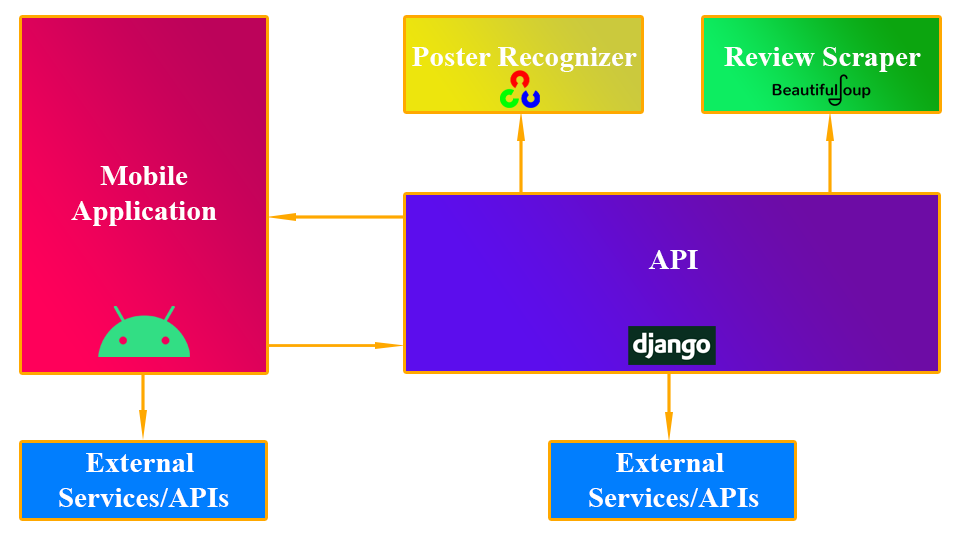
\includegraphics[width=450px]{templateLaTeX-Eng/img/conceptualArchitecture.png}
        \caption{\bf Conceptual architecture of the system.}
    \end{center}
\end{figure}

The conceptual architecture is presented by Figure 5.3. It is comprised of the following modules:
\begin{itemize}
    \item Poster Recognizer: OpenCV application written in Python that receives user submitted photos of movie posters and identifies and returns the title of the movie in question.
    \item Review Scrapers: Python application that uses Beautiful Soup in order to scour the web for movie reviews given its title or identification code.
    \item External Services/APIs: These are already existing systems with functionalities that benefit our system and that wouldn't make sense having a separate and custom implementation for. Some of the functionalities provided by them are: authentication using external platforms, movie databases, poster databases.
    \item API: Web server implemented in Python using the Django framework that exposes the functionalities of the previous modules through its endpoints. 
    \item Mobile Application: Android mobile application written in Kotlin that makes use of the API and other external services through HTTP requests to achieve the overall purpose of the project. It also serves as the user interface of the system.
\end{itemize}

%=======================================================================================================  

\section{Used Technologies}
This section will present the main technologies, programming languages, tools, libraries and frameworks that went into making the thesis project. This is not meant to be an exhaustive list, as mentioning every library used would be overkill.

\subsection{Python}
Python is one of the programming languages that will be needed to develop the system. The modules that will be written in python are the poster recognizer, the web scraper and the Django API. It is high-level, object oriented programming language that was designed to be simple and portable. It strongly encourages modularity and code reuse, and can be run on almost any platform. 

Python is has a very large number of applications, maybe more than any other programming language out there. It offers many packages for web development and integration with numerous internet protocols. It is also widely used in data processing and numeric computing, making it great for image processing.

\subsection{PyCharm}
PyCharm is an IDE, which is short for Integrated Development Environment, that was desgined specifically for Python. Being developed by JetBrains, it is very similar to other popular IDEs developed by them, like IntelliJ and Android Studio, which we'll talk about later. Since it supports all the major libraries Python has to offer, using it is a no-brainer. 

Among it's many features, some worth mentioning are: coding assistance and analysis, curtesy of IntelliSense, which allows for code completion, error and syntax highlighting, efficient refactoring, support for web development and a very beautiful and easy to use UI, among many others.

\subsection{OpenCV}
The OpenCV library was presented more in depth in previous chapters. Since a part of our project has to do with image processing, a suitable library that can perform operations on images is needed. The vast array of advantages that OpenCV has to offer were discussed in chapter 4, as well as the why the Python version of the library was chosen.

\subsection{Beautiful Soup} 
One of the most popular web scraping libraries, Beautiful Soup is best used to build small scale, quick and efficient web crawlers. A more in depth description of the library is given in chapter 4 of this paper.

\subsection{Django}
The framework of choice that was used to build the web API is Django. The fact that it is written in Python means that integration with the other Python modules can be done seamlessly, without the need of any extra communication that would lead to a lower performance. The simplicity and efficient structure of Django is one of it's main attractions.

\subsection{Kotlin}
For a while, Java was the only language used to develop Android applications, until 2015. That year Google introduced Kotlin, because of the need to solve many design issued that came with Java and to improve the overall development process.

Kotlin is a statically typed programming language that offers typer inference, null safety and many other attractive features. In 2018, it was the fastest gorwing language on GitHub and it has risen to the fourth place in the "most loved programming languages" ranking done in 2020. The clean and compact syntax the language offers helps developers create more high quality applications, less error prone, with easier maintenance and modifiability. It provides many functionalities Java lacks, like operator overloading, data classes and extension functions, as well as getting rid of the dreaded semicolon.

Many big companies have made the switch from Java to Kotlin and it has paid off. Developers seem to be more satisfied and this shows in the quality of their products. I will be following their lead by implementing my application in Kotlin as well.

\subsection{Android Studio}
Android Studio is the official IDE used for Android development, which is endorsed by Google. It was built on JetBrain's IntelliJ so many of the features we have seen in PyCharm are present here as well. Due to its similarity with PyCharm, the transition from one project to another won't be as jarring and the development process will go smoother. 

Among the many advantageous features the IDE has, some worth mentioning are: IntelliSense, the code assistance software, Grade build support, support for Android apps on any device (smartwatch, tv, car, etc.), Android specific refactoring tools and the ever-present intuitive design all JetBrains IDEs have.

\subsection{Git}
Last but not least, a version-control system is needed for tracking and improving the development process. While most commonly used within software development teams, the tool is great for managing solo projects as well. 

By keeping track of all modifications, mistakes and bugs can be more easily solved. Version control also allows to bring the project to a previous version, scrap unwanted changes easily and an easy and efficient way of backing up the code base. Git has become an essential part of any software project.

I will be using Gitlab as my Git repository manager and Sourcetree as the Git client which provides a GUI of my repositories and makes the overall development process easier.

%=======================================================================================================  

\section{Poster Detection Pipeline}
The first step in the implementation of the image search of our system is to detect where the poster resides in the photo received from the user. To do this, I have devised a pipeline that will manipulate the input picture and convert it so that the poster can be identified.

Before we go into the image processing itself, we need to open the image and convert it to a for which OpenCV is familiar with. OpenCV has a function that loads an image from a file and returns an image in the form of a matrix. Each element from the matrix represents a pixel. With imread, we can open an image in many modes, the most popular of which are color and grayscale.

Now that we have our image, it's time to start applying operations on it. In order to detect a poster, we will first find the edges of the poster. Knowing that any poster has a rectangular shape and a size ration of approximately 2:3, we can start by finding all the rectangular shapes present in the photo. Of course, the perspective might be skewed, making our poster have a diamond-like shape. 

In chapter 4, we described how Canny Edge Detection works and that it is a suitable algorithm for the problem at hand. We have also discussed that some preprocessing steps must be taken to achieve the best performance of John F. Canny's algorithm.

As most algorithms, Canny requires a grayscale image. This means that all pixels must have a single value between 0 and 255. So the first step in our pipeline is to convert our color image to grayscale. OpenCV provides the cvtColor function, in this regard. It requires two parameters, the image itself and a flag that indicates the desired outcome, in our case COLOR\_BGR2GRAY.

Next, we should apply a blur effect to achieve better edges. The GaussianBlur function, as it name suggests, is used to add a Gaussian Blur to images. After that, we need to convert the image to a black and white image, or a binary image. The threshold function does this by applying a thresholding operation to our image.

At this point, morphological operations can be applied to the image. Even though there are 4 operations we are interested in, I found that a simple closing operations suffices in order to define better edges. The morphologyEx function is used for morphological operations. In our case the parameters will be: the image itself, a flag that indicates that we want to perform a closing operation, that is MORPH\_CLOSE, and a closing kernel, in this case of size 5x5.

Now that all the required steps to perform the edge detection have been taken, the Canny Edge Detection can work its magic. Fortunately, OpenCV already provides an implementation of the algorithm, through its function properly named Canny. This helps us avoid "reinventing the wheel". Until now our code looks like this: 
\begin{lstlisting}[language=Python]
import cv2

# Convert image to grayscale
grayscaleImage = cv2.cvtColor(originalImage, cv2.COLOR_BGR2GRAY)

# Blur image for better edges
blurredImage = cv2.GaussianBlur(grayscaleImage, (7, 7), 0)

# Apply threshold
ret, thresholdedImage = 
    cv2.threshold(blurredImage, 127, 255, cv2.THRESH_BINARY)

# Apply closing
closingKernel = np.ones((5, 5), np.uint8)
closingImage = 
    cv2.morphologyEx(thresholdedImage, cv2.MORPH_CLOSE, closingKernel)

# Canny Edge Detection
cannyMinVal = 100, cannyMaxVal = 200 # values could vary
cannyImage = cv2.Canny(closingImage, cannyMinVal, cannyMaxVal)
\end{lstlisting}

Having defined and detected the edges of the photo, we should now identify which ones represent the poster. As stated in chapter 4, there are two important features we are looking for in a contour: that it has a closed perimeter and that it has exactly 4 sharp corners. Also, if the perimeter is small, we can safely assume that the contour does not constitute a poster, as the poster should be the focus of the photo.

The findContours OpenCV function can isolate each contour and return a list of contours represented by an array of pixels. This way we can start analyzing each contour by iterating the list. First, we need to calculate the perimeter of the contour, which can be done with the function arcLength. If the perimeter is too small, we can discard it and go on to the next. Otherwise, we can structurally analyze the shape of the contour with the function approxPolyDP. This approximate the polygonal curves of the contour. From this, we can check whether the contour has 4 corners.

After we have identified all the contours that have a rectangular shape, we should determine which one is the actual poster. As we stated before, it is assumed that the user will provide a photo in which the poster is the central element. Thus, we can safely assume that the contour with the largest area will constitute our poster. Calculating the are is fairly easy, as OpenCV provides us with the function contourArea.

 \begin{figure}[H]
    \begin{center}
        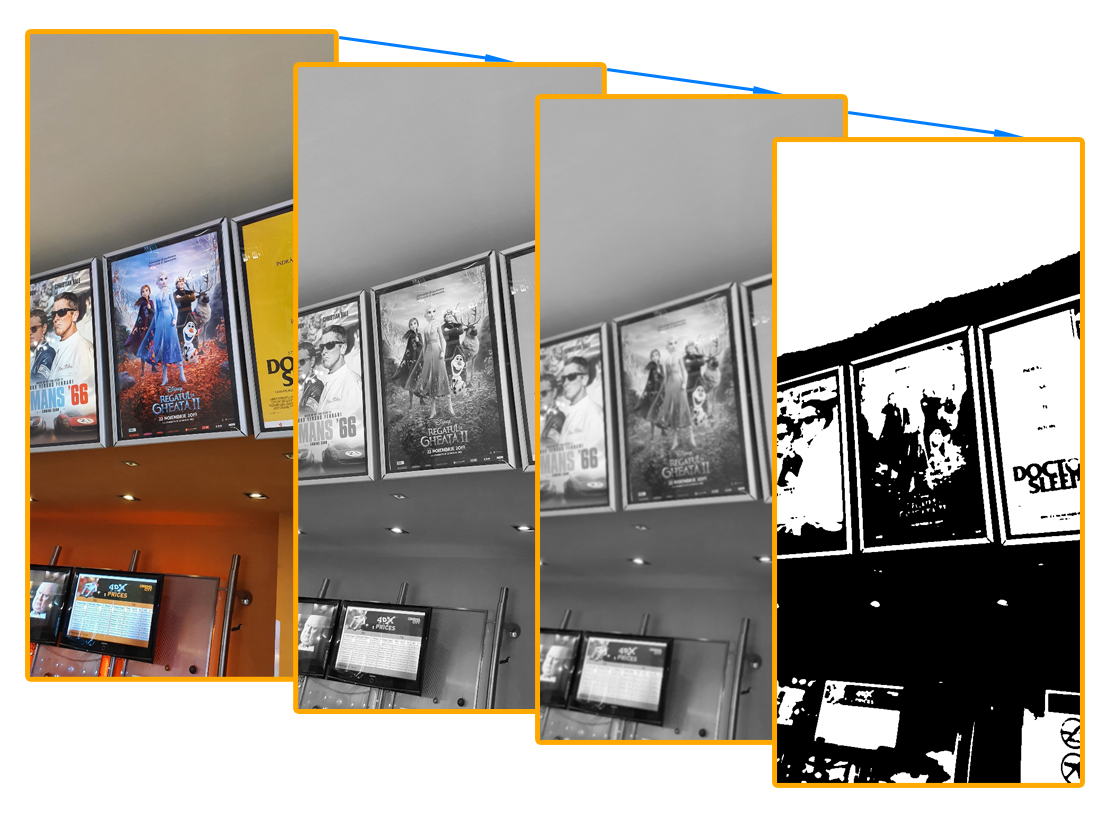
\includegraphics[width=410px]{templateLaTeX-Eng/img/posterdetection1.png}
        \caption{\bf Poster detection pipeline (Part 1).}
    \end{center}
\end{figure}

Having identified the poster, a perspective transformation will be applied. The user isn't expected to provide a photo that with a perpendicular point of view of the poster. Thus, the poster will be skewed. The OpenCV function, warpPerspective applies a perspective transformation images. The only other calculations we need to perform is determining the source and the destination points. This is easy, as we have the corners of the poster from a previous step.

 \begin{figure}[H]
    \begin{center}
        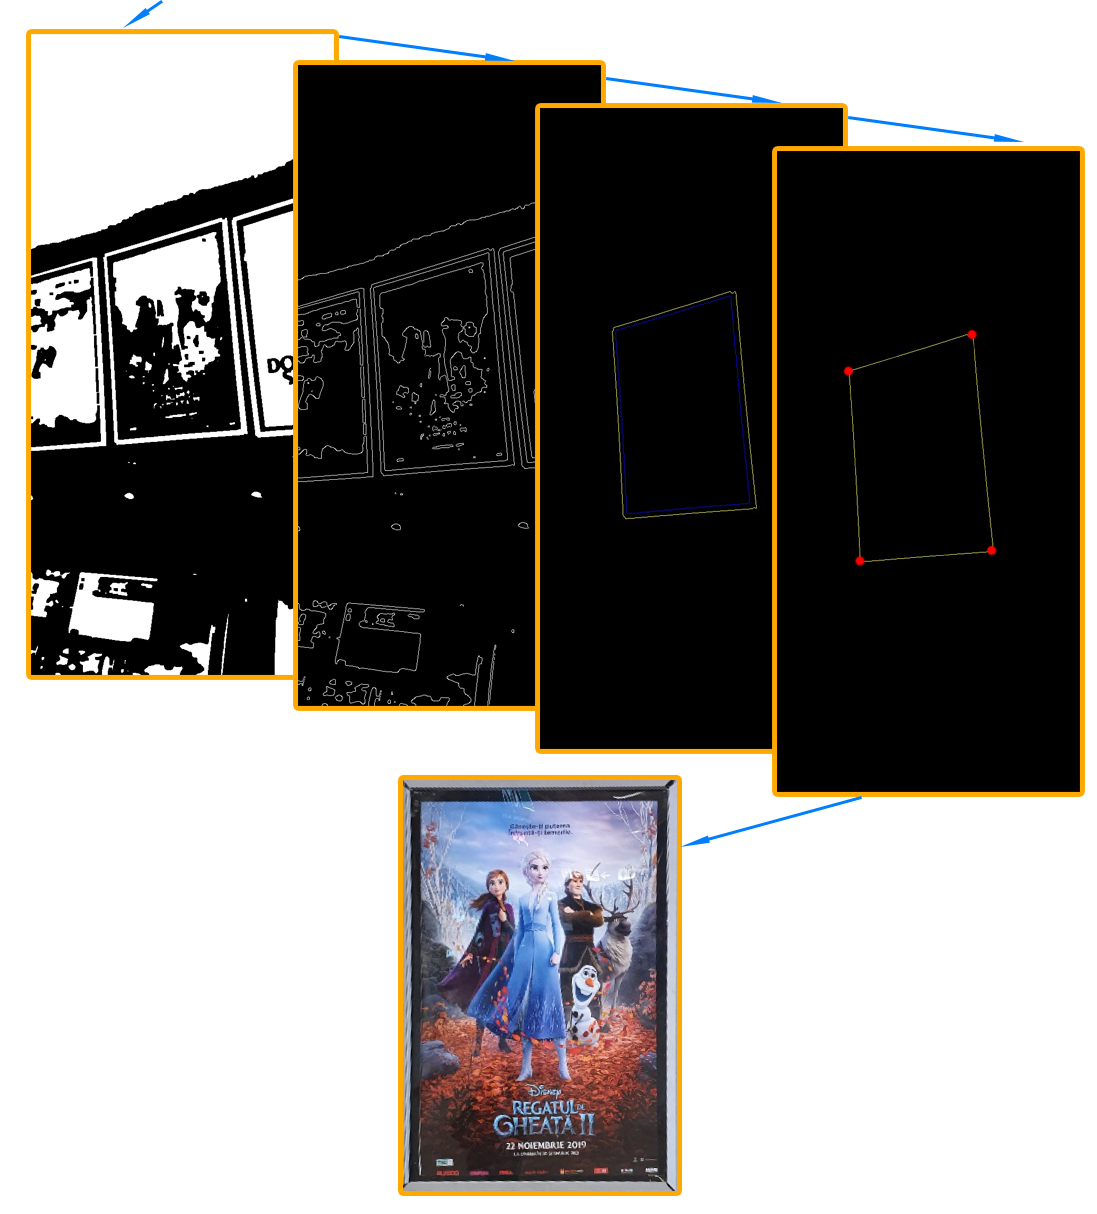
\includegraphics[width=410px]{templateLaTeX-Eng/img/posterdetection2.png}
        \caption{\bf Poster detection pipeline (Part 2).}
    \end{center}
\end{figure}

%=======================================================================================================  

\section{Poster Recognition}
Having extracted the actual poster from the user submitted photo, we now have to identify the actual movie depicted in the poster. The approach I have chosen consists of keeping a database of all the posters with their movie titles. Next, the extracted poster will be compared against the posters stored in that database, and when there's a good enough match, the movie title corresponding to that poster will be returned. Of course, since there exist over 500,000 movies, each having at least one poster, it would be unpractical iterate through all of the database. While this problem is still a work in progress, the current implementation only incorporates the most popular movies and the movies that are in cinema now. This decision comes from the fact that the image search aspect of the system is meant to be used by people who are at the mall, and in the spur of the moment decide to watch a movie and taking a picture of the displayed posters is faster than manually typing all the titles. 

The recognition itself consists of image comparisons. We will compare the extracted poster with actual movie posters and compute a comparison metric. All the metrics resulted will be compared and the best match will be returned.

One of the best features of images to compare is color. The first thing that pops in an image to the human eye is its colors. The color structure and distribution can tell a lot about the picture's content. This brings us to hsitograms. In previous chapters, we discussed what histograms are and why they are so important. To get caught up, histograms represent the distribution of pixel values across an image. They basically plot what colors are present in the image and how often they appear.

Comparing histograms is one of the best operations to perform when deciding whether two images are similar. If their histograms match, there's a high chance the images are the same. In this regard, there's a lot of histogram comparison methods which use different metrics to compute how well histograms match. These are: Correlation, Chi-Square, Intersection and Bhattacharyya. Since our picture may not accurately represent the poster, it is best to calculate the histograms in the HSV color space.

OpenCV provides us with the proper functions to achieve this. To convert the image to HSV, the previously mentioned cvtColor function can be used with the COLOR\_BGR2HSV flag. Then, the function calcHist can be used to calculate the histogram. For better histogram data, they can be normalized using the normalize function.

There are two more improvements we can do before the histogram comparison. The first one is to equallize the histograms to make them more uniform. The second improvement can be done before all the other operations. We can split the image into regions and calculate and compare the histograms by region. This will give us a better comparison if some part of the extracted poster has glare, noise or is corrupted in any other way.

For the comparison itself, OpenCV has the compareHist function, which receives the two histograms to compare and a flag that designates all the comparison methods available. These are: HISTCMP\_CORREL, HISTCMP\_CHISQR, HISTCMP\_INTERSECT and HISTCMP\_BHATTACHARYYA. We are interested in all the comparison methods. The function will return a metric specific to each comparison method. We can analyze and even average the metrics accordingly to get a better clue of how much the images actually resemble each other.

Finally, by comparing all the resulted data, we can find what poster better matches our picture. The corresponding movie title to the poster will be returned.

%=======================================================================================================  

\section{Using Existing APIs}
Using existing APIs is very useful. They can provide data and functionalities that can be very hard to achieve from scratch. In our case, fetching information on movies, of which there are over 500,000 of, is an almost impossible task. 

IMDb, or the Internet Movie Database, as its name suggests, is an online database containing data about films, television and other media content. Having information like cast, production, plot summaries and reviews, IMDb is the go-to website for information on any type of media.

Since we need a way to gather movies and acces information about them, IMDb seems a great place to start. Unfortunately, the IMDb API is very hard to use. For starters, there isn't an online documentation available. Also, getting an API key is a very convoluted process and some payment is needed. Due to the difficulty of accessing the IMDb API, we will discard it for now. 

Having ruled out the IMDb API, I had to find other suitable API to achieve the purpose of the project.

\subsection{OMDb API}

The Open Movie Database API [23] is a RESTful web service containing information about movies that is kept up to date and is maintained regularly. The developers that created this API made it available for free, which already gives it an edge over the IMDb API. 
While it has many endpoints, each having a unique functionality, there are a few we are interested in. The first one, seen in used in Figure 5.6, is the search endpoint. With its single parameter being "s", through which keywords of a movie's title must be passed, one can request a list of search results that match that parameter. The response takes the form of a JSON which contains a list of search results. The search results contain information such as the title and release year of the movie but, most interesting is that it also includes an ID that corresponds to IMDb.
 \begin{figure}[H]
    \begin{center}
        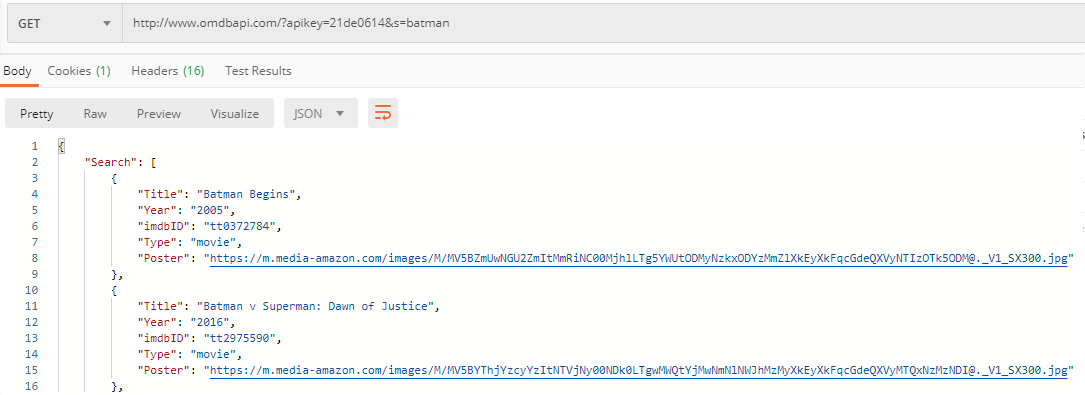
\includegraphics[width=450px]{templateLaTeX-Eng/img/searchendpoint.png}
        \caption{\bf Search endpoint of OMDb.}
    \end{center}
\end{figure}

The second important endpoint we can use is the one represented in figure 5.7. It can also be accessed through a GET request although the parameter used is "i", and it represents an IMDb id. Coupled with the previous request, this can be used to retrieve detailed information about a movie. Data like the cast, crew, plot, box office earnings and ratings can be retrieved through a request to this enpoint.

 \begin{figure}[H]
    \begin{center}
        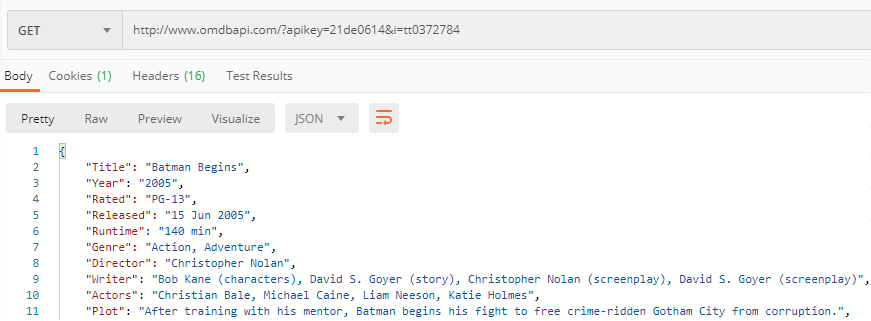
\includegraphics[width=450px]{templateLaTeX-Eng/img/getendpoint.png}
        \caption{\bf Request for getting detailed information about a movie through OMDb.}
    \end{center}
\end{figure}
\footnotetext{The figures in this page do not display the entirety of the HTTP responses.}

\noindent The OMDb API will be the main service that will be used in the mobile application.

\subsection{TMDb API}
The Movie Database API [24] is an API similar to OMDb. Although it offers many more endpoints than the latter, it is a bit overkill to use it in our project. However, there are some endpoints we are interested in.

The "/movie/popular" endpoint retrieves the the most popular movies of the current day. This will be used to give the user an idea of what other people like. The "movie/\{tmdbId\}/recommendations"endpoint gets movie recommendations based on an id. That id represents a certain movie and the recommendations provided will be similar to said movie. The third endpoint is only needed to retrieve the TMDb id of a movie through its IMDb id. Since OMDb works with IMDb ids and TMDb works with TMDb ids, we need a way to link the two. This endpoint helps us achieve this.

%=======================================================================================================  

\section{Movie Review Web Scraping}
We have discussed what web scraping is and how it works in previous chapters. This section will present how the BeautifulSoup library will be used to fetch and aggregate movie reviews. 

The first step is to analyze the structure of a review. All reviews have a title, which shows the reader what to expect, a rating, which quantifies how likely the reviewer is to recommend the movie and the review itself, which is just text. Additionally, the review may contain spoilers, which must be dealt with. Thus, another element of a review is a flag that indicates whether the review contains spoilers or not. 

Having identified the important elements of a review, it is time do so some web scraping.

\subsection{IMDb Crawler}
The first and most important source we want to focus on is IMDb [25]. As stated before, IMDb is possibly the most popular and everyone's first choice when searching for information on a movie. The website also contains user and critic reviews, which is our point of interest.

First, we need to make a GET request to the page of the movie we want to fetch reviews of. This is easily done with the \textit{requests} Python module. Using the \textit{get} function of the \textit{requests} package, we are able to retrieve all the information of that page. We are interested in the HTML code, which can be accessed through the \textit{text} attribute.

The extracted HTML code is then passed to the \textit{BeautifulSoup} constructor, along with the type of parser we want to use, in our case \textit{lxml}. This will turn the HTML document into a parsable tree. The next step is to find where the reviews are in the tree. This is done by analyzing the webpage with the developer tools of browsers. As stated in a previous chapter, most of the time spent in web scraping, is spent in the browser rather than actually coding. 

 \begin{figure}[H]
    \begin{center}
        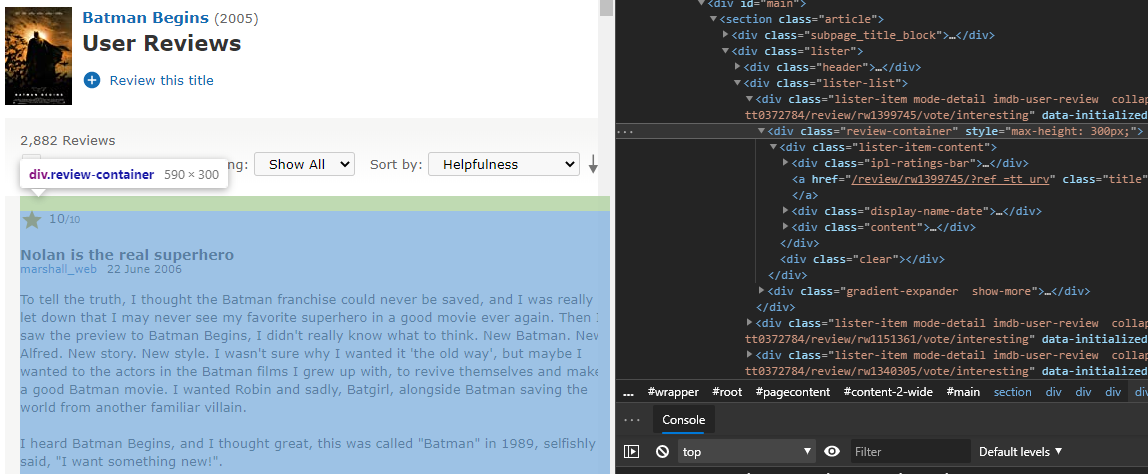
\includegraphics[width=450px]{templateLaTeX-Eng/img/browsertools.png}
        \caption{\bf Using the browser's developer tools.}
    \end{center}
\end{figure}

In the figure above, it can be observed that each review is enclosed in a \textit{div} with the class type \texit{review-container}. Thus, we have to iterate through all of the \textit{divs} that have that class type and retrieve the data they contain through similar processes.

From the extracted data, a JSON object will be constructed, containing all of the reviews.

\subsection{Metacritic Crawler}
A very important and highly respected website we are interested in is Metacritic. Many people end up on Metacritic in order to see the value of a movie. The website also aggregates reviews from well known critics so it is essential to fetch reviews from there.

Accessing the Metacritic page of a movie is a little bit more difficult than it was on IMDb. For IMDb we could use the \textit{imdbId} we received from the OMDb API. Metacritic, however, does not use those. A workaround would be to access the Metacritic website through the IMDb page. After a close analysis of IMDb, I observed that there is a hyperlink on each movie page, to the corresponding page on Metacritic.

Thus. the \textit{requests} package can be used once for retrieving the IMDb page, and after finding the exact location and structure of the Metacritic hyperlink, once more to retrieve the HTML page of Metacritic. 
After reaching and retrieving the Metacritic, similarly to the IMDb crawler, the review containers will be found and their data will be extracted. After that, the reviews will be appended to the JSON constructed previously.

%=======================================================================================================  

\section{Building a Django API}

Although Django is a very complex framework, with a myriad of features and resources to build web applications, we will only use a small part of what it has to offer. Since we do not need a GUI for our web application, we will only focus on the \textit{view.py} and \textit{urls.py} files. 

Firstly, we need to incorporate our two previous components in the Django project, the poster recognizer and the web crawlers. This is simply done by creating separate packages for them and fixing some imports. Since they are Python applications, no other configurations must be done.

In the \texit{urls.py}, the endpoints must be defined. The two main endpoints of the application are: \texit{/reviews/\{imdbId\}/} and \texit{/imageSearch/}. The first one will be used to fetch reviews of a particular move through its IMDb id and the second one will perform the poster recognition algorithm and will return the movie's title.

In addition to those endpoints, I also created two other endpoints that make use of the TMDb API. These are: \texit{/popular/} and \texit{/recommended/\{imdbId\}}. They are used for retrieving the current day's most popular movies and recommendations based on a given movie. The reason why the TMDb API wasn't used directly in the client applications will be detailed in a future section.

The\textit{views.py} will define what each endpoint should do. Each class in this file handles the HTTP requests as they come in. Firstly, they define what type of HTTP request it is: GET, POST, PUT or DELETE. Afterwards, they read the request's content: header, body, etc. and validate the data. With the data from the request, if valid, the corresponding operations can be performed. Finally, a HTTP response that has the outcome of each operation, in the form of JSONs, is build and returned.

Django handles all the communication infrastructure, all the security parameters and most of the hard work for the programmed. Of course, developers with serious project can choose to modify all of those aspects but in my case, it is not in the scope of the project.

%=======================================================================================================  

\section{Deploying the API}
Heroku [25] is a cloud platform as a service (PaaS) that allows developers to host their application without worrying about all the complex infrastructure aspects. It offers a free plan, which is ideal for deployment of experimental, small scale applications. In our case, we need to deploy a simple Django API with a reduced number of endpoints. For the scope of this project, the performance of the web service isn't a concern.

While, initially, Heroku was build only for Ruby applications, the massive success of the platform allowed for the development of support of other programming languages. Among them, Python is listed as a compatible technology.

Deploying our Django API on Heroku is as simple as creating an account, installing the Heroku Command Line Interface (CLI) and creating a Heroku git repository containing the application. Additionally, the repository must contain a \textit{requirements.txt} file, which defines all the Python libraries needed to run the Django project. When the repository is created, a Heroku application is created with it. Through this application, developers can manage all the deployment aspects, such as name, base url, logs and plugins. 

After the Django application is up and running on the cloud platform, each push of the local changes causes the remote project to be rebuilt and redeployed. One must be careful to keep the \textit{requirements.txt} file up to date, otherwise, unexpected crashes might occur.

 \begin{figure}[H]
    \begin{center}
        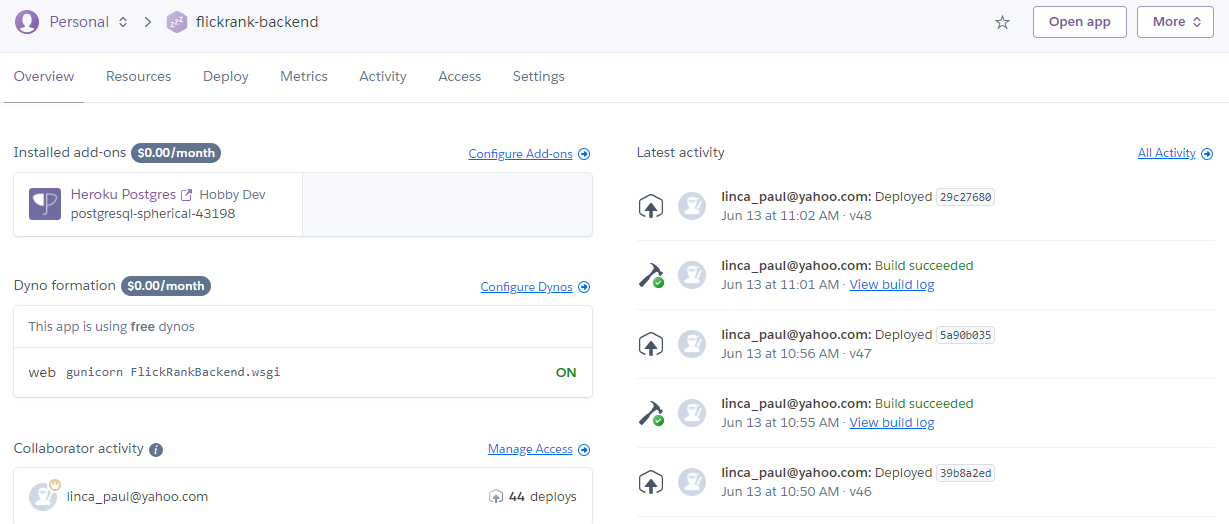
\includegraphics[width=450px]{templateLaTeX-Eng/img/herokudashboard.png}
        \caption{\bf Heroku dashboard used for managing the deployed application.}
    \end{center}
\end{figure}

The API can be found online at https://flickrank-backend.herokuapp.com/ with the following endpoints:
\begin{itemize}
    \item reviews/<slug:imdbId>
    \item popular/
    \item recommended/<slug:imdbId>
    \item imageSearch/
\end{itemize}
\pagebreak

%=======================================================================================================  

\section{FlickRank}
The name of the Android application developed in the context of this project is FlickRank. By combining the two main concepts encapsulated in the app, "flick", meaning motion picture or movie, and "rank", meaning to class, order or classify, the purpose of the project can be derived from its name. The purpose of the FlickRank app is to allow the user to search for movies and provide them with an aggregation of reviews.

The application was developed using the Kotlin language. As more and more developers and companies make the switch from Java to Kotlin, the general-purpose language has quickly become one of the most loved programming languages of the current century. It is continuously tweaked and improved and a myriad of resources, documentations, tutorials and forums can be accessed for a better development process. The Kotlin community has grown exponentially in the last years and even Google announced it as the official Android development language

The features and main functionalities of the application will be presented in the following sections.

%=======================================================================================================  

\section{Authentication and Firebase}
Users will need to authenticate into the application in order to use it. This will provide a secure and more personalized experience. It is well known that most users dread the process of creating yet another account, with its own password to remember. This is why most platforms today opted for another alternative.

Firebase [26] is a development platform for mobile and web applications. Acquired by Google in 2011, the platform provides many services developers can use to enhance their projects. Some of the solutions featured by Firebase are: Analytics, Cloud Messaging, Database and Cloud storage, hosting, testing and many more stability and performance boosters. The one we are concerned with, though, is Firebase Authentication. 

Firebase authentication is an authentication service that lets the developers choose how users can log into their application. While app-specific accounts are supported by the service, we have already state that that is the wrong way to go. 

Perhaps the most useful feature Firebase has to offer is their support for social login providers. This means that authentication can be done through already existing accounts on other platforms, such as Facebook, Google, Twitter and GitHub. This feature directly ties into the main themes of mu thesis project. The convenience factor comes from removing the need of creating a new, separate account, while giving users the option of authentication with a single tap through their already existing Google account. 

Since Google owns both Firebase and Android, integrating the Firebase into our application is smooth and straight forward. The process consists of registering the application with the Firebase Console and Android Studio will directly add the required dependencies to the Android project. 

From here, a Google log in button is added in the corresponding log in page and the standard authentication code provided in the Firebase documentation. Upon tapping the button, the user will be prompted with a dialog and asked to choose which Google account should be used for authentication. After choosing, all the app's features will be available to the user.
 \begin{figure}[H]
    \begin{center}
        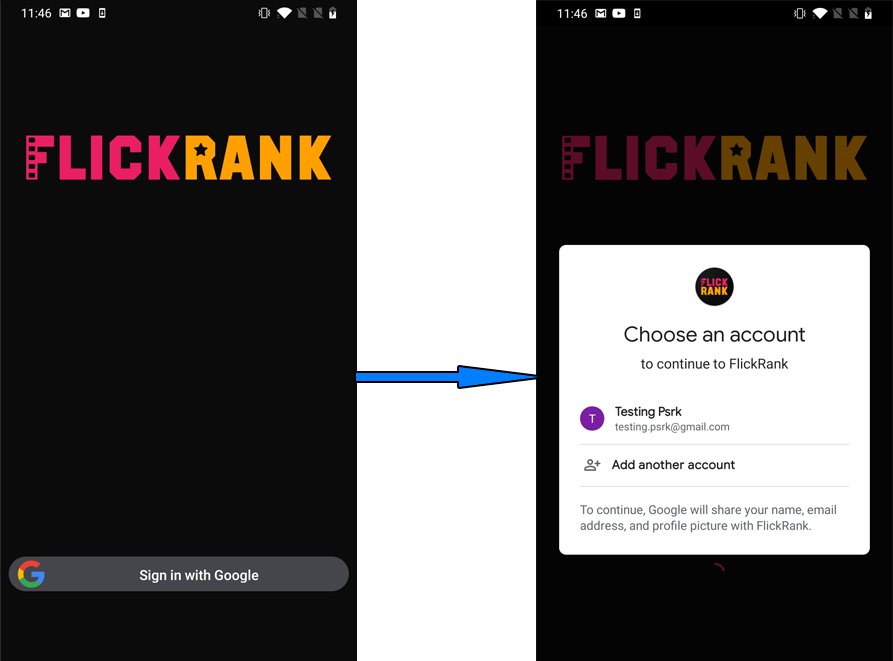
\includegraphics[width=400px]{templateLaTeX-Eng/img/auth.png}
        \caption{\bf The application's authentication process.}
    \end{center}
\end{figure}

%=======================================================================================================  

\section{Application Structure}
The application is divided into tabs, each one providing specific functionalities for the user. There are three main tabs:
\begin{itemize}
    \item Settings: This tab allows the user to clear personal information as well as log out of the application.
    \item Discover: The discover tab displays to the user their view history as well as recommendations in the form of the day's most popular movies and similar movies to the ones contained in the search history.
    \item Search: The search tab is the most complex one. It handles the search aspect of the application. The user is prompted with two search modes: manual and image search. Manual search consists in the user typing the movie title in the search box. The image search is split into two additional alternatives: taking a photo with the device's camera and choosing an already existing photo from the phone's storage.
\end{itemize}
 \begin{figure}[H]
    \begin{center}
        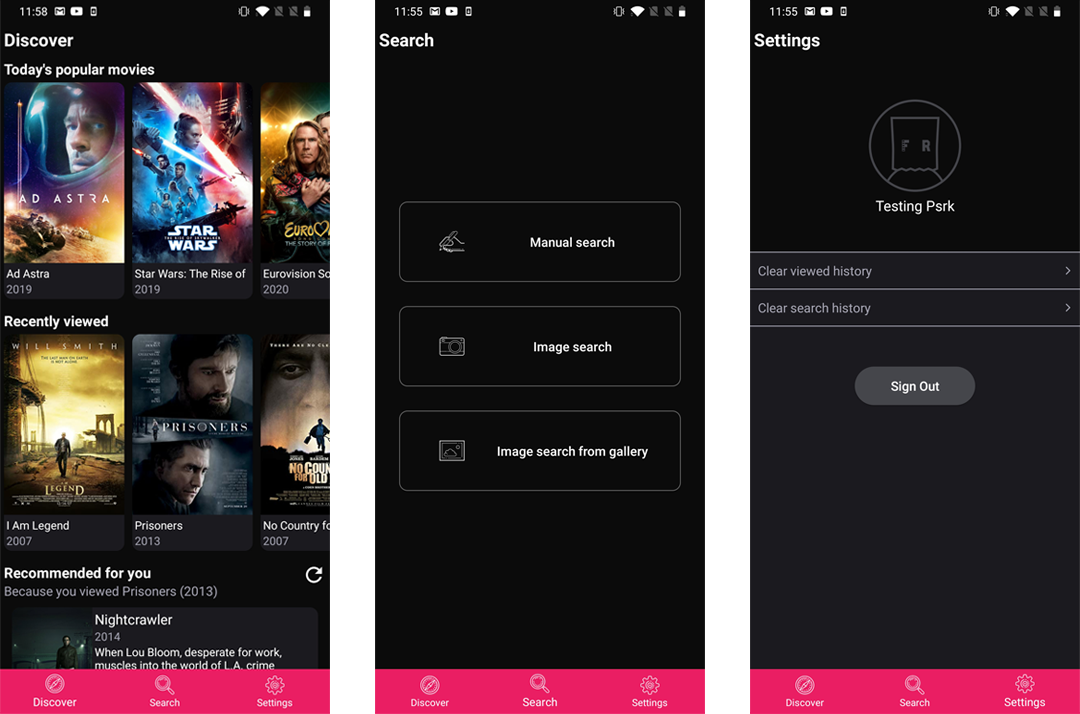
\includegraphics[width=410px]{templateLaTeX-Eng/img/tabs.png}
        \caption{\bf The application's main tabs.}
    \end{center}
\end{figure}

%=======================================================================================================  

\section{Application Architecture}
The way a project is structured is its most important aspect. This is no exception when it comes to Android applications. Properly designing and implementing the application's architecture makes it more scalable and maintainable. Programmers less time building the project then they do maintaining it and bug fixing.

\subsection{MVVM}
The solution most Android developers employ is the MVVM patter, or the Model-View-ViewModel pattern. This pattern's popularity comes from the great results it delivers. The main advantages of the MVVM pattern are:
\begin{itemize}
    \item Great separation of concerns and responsibilities throughout its components, which leads to low-coupling and high-cohesion. ViewModels don't hold any reference to the View, as is the case in the closely related MVP pattern.
    \item Provides better performance and a more organized and easy to understand development process.
    \item Modifications are more easily implemented because of its independent components.
    \item Increased testability.
    \item Support for automatic data binding between the View and the ViewModel.
\end{itemize}

\noindent The components of the MVVM pattern are:
\begin{itemize}
    \item View: Represents the graphical interface presented to the user. It handles user input.
    \item ViewModel: Keeps track of the states of the data, which is observed by the View. Usually, it contains a Binder that notifies the View of any state change. Thus, the View can update it's interface.
    \item Model: Represents the data that is observed. It's sole purpose is to represent and store data and information.
\end{itemize}

 \begin{figure}[H]
    \begin{center}
        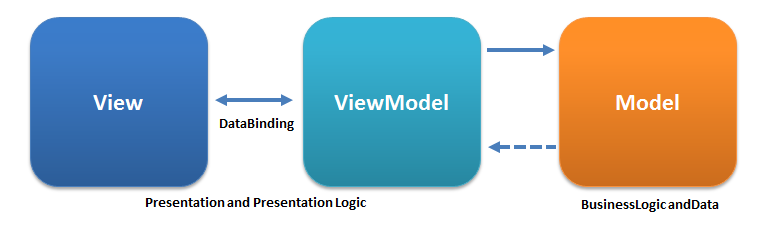
\includegraphics[width=410px]{templateLaTeX-Eng/img/mvvm.png}
        \caption{\bf MVVM components\footnotemark}
    \end{center}
\end{figure}
\footnotetext{Source: https://en.wikipedia.org/wiki/Model\%E2\%80\%93view\%E2\%80\%93viewmodel}

\subsection{Dependency Injection with Koin}
Dependency injection is a technique that passes objects all the objects it needs, i.e. its dependencies. This relieves the programmer from manually providing them, considerably reducing the amount of code that has to be written. The coupling is also significantly reduced between components. 

Koin is a relatively new dependency injection framework for Kotlin. Even so, it has dethroned Dagger as the go-to dependency injection framework, due to its lightweight, simplicity, performance and vast array of functionalities. 

The Koin module we are most interested in is the \texit{koin-android-viewmodel}. It provides developers the chance to implement the MVVM as efficiently as possible. It is used to inject the ViewModel components to the corresponding Views. It also facilitates storing the state of the screens upon navigating away from them, as it can make the ViewModels singletons. Thus, the ViewModel won't be initialized every time a page is accessed. 

%======================================================================================================= 

\section{Consuming RESTful Services with Retrofit}
We have established that the mobile client will make use of the Django API we created, as well as the OMDb API. Thus, we need a way make HTTP calls from our application.

Retrofit is a REST client used for consuming RESTful web services in Android. It is a powerful framework for interacting with APIs by sending requests with the help of OkHttp. The library automatically consumes JSON and XML responses and parses them into Plain Old Java Objects (POJOs).

What needs to be defined in order to work with Retrofit are the three following classes:
\begin{itemize}
    \item The data model classes that represent the objects received from the requests as JSON.
    \item The interfaces that define all the needed HTTP operations.
    \item The \textit{Retrofit.Builder} class that instantiate the main object that will perform the HTTP requests and will map the JSON responses to the corresponding data models. 
\end{itemize}

 \begin{figure}[H]
    \begin{center}
        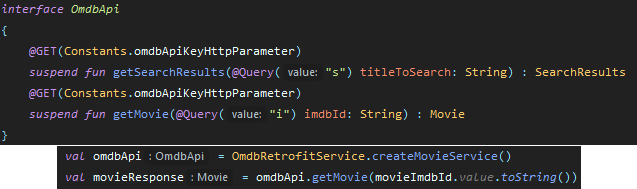
\includegraphics[width=450px]{templateLaTeX-Eng/img/httprequest.png}
        \caption{\bf Example of using Retrofit for making requests to the OMDb API.}
    \end{center}
\end{figure}

%======================================================================================================= 

\section{Mobile Application Design}
The Android application is broken down into many packages, each one having a specific function.
 \begin{figure}[H]
    \begin{center}
        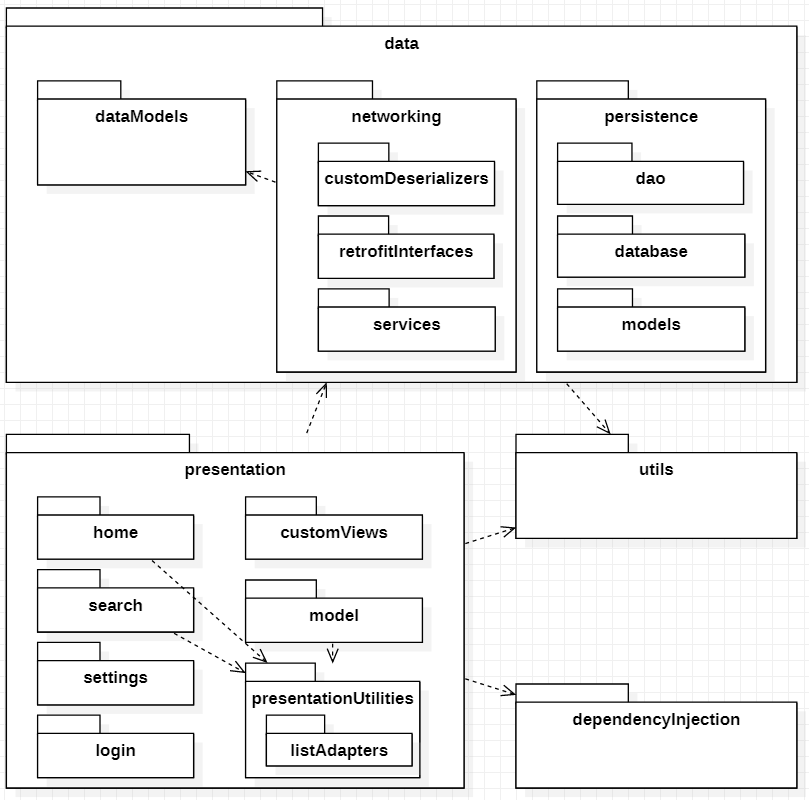
\includegraphics[width=450px]{templateLaTeX-Eng/img/packagediagram.png}
        \caption{\bf The mobile application's packet diagram.}
    \end{center}
\end{figure}
\pagebreak

Here's how the classes are associated and work with each other in order to perform the search operation:
 \begin{figure}[H]
    \begin{center}
        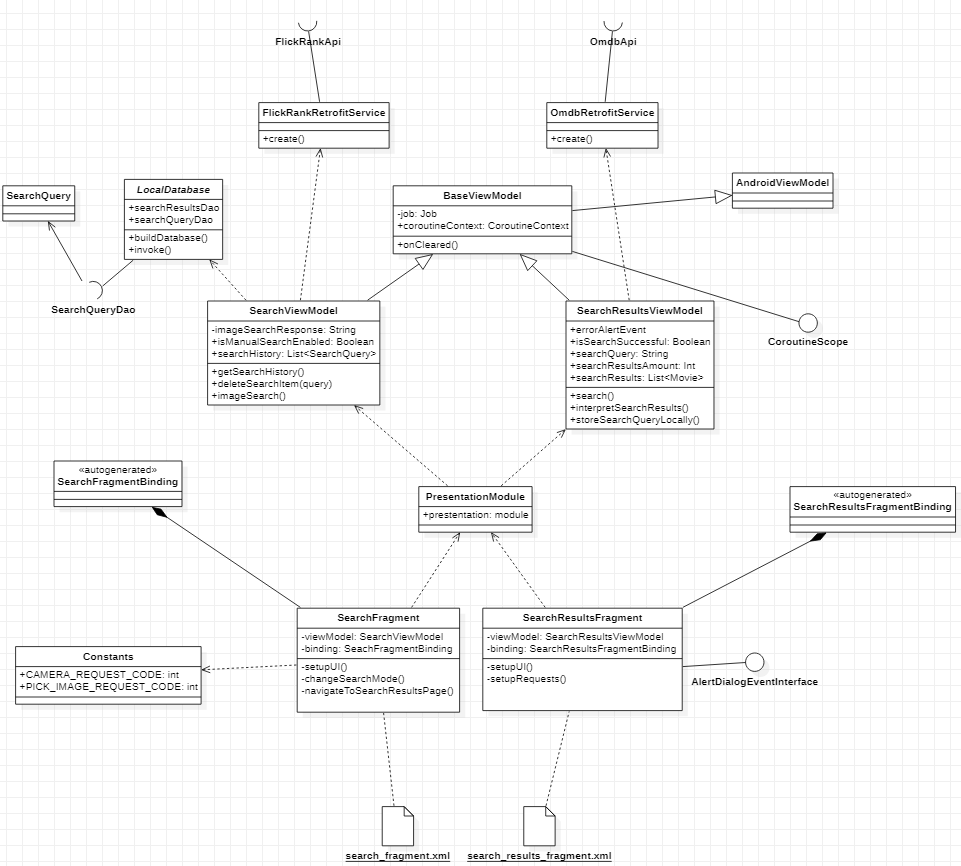
\includegraphics[width=500px]{templateLaTeX-Eng/img/classdiagram.png}
        \caption{\bf Partial class diagram of the components used in the search operation.}
    \end{center}
\end{figure}
\pagebreak

\chapter{Testing and Validation}
The development process of this project has proven itself to be very difficult. Having that many components interacting with each other be developed by a single person can create many unwanted scenarios. Any malfunction in any of the components can be detrimental to the whole system.

During the development of the poster recognition component, all the intermediary results were tested as they were implemented. Having a small set of testing photos and a large array of possible, unexpected environmental factors that could affect the algorithm may have left this component incomplete. Even so, the results were satisfactory.
 \begin{figure}[H]
    \begin{center}
        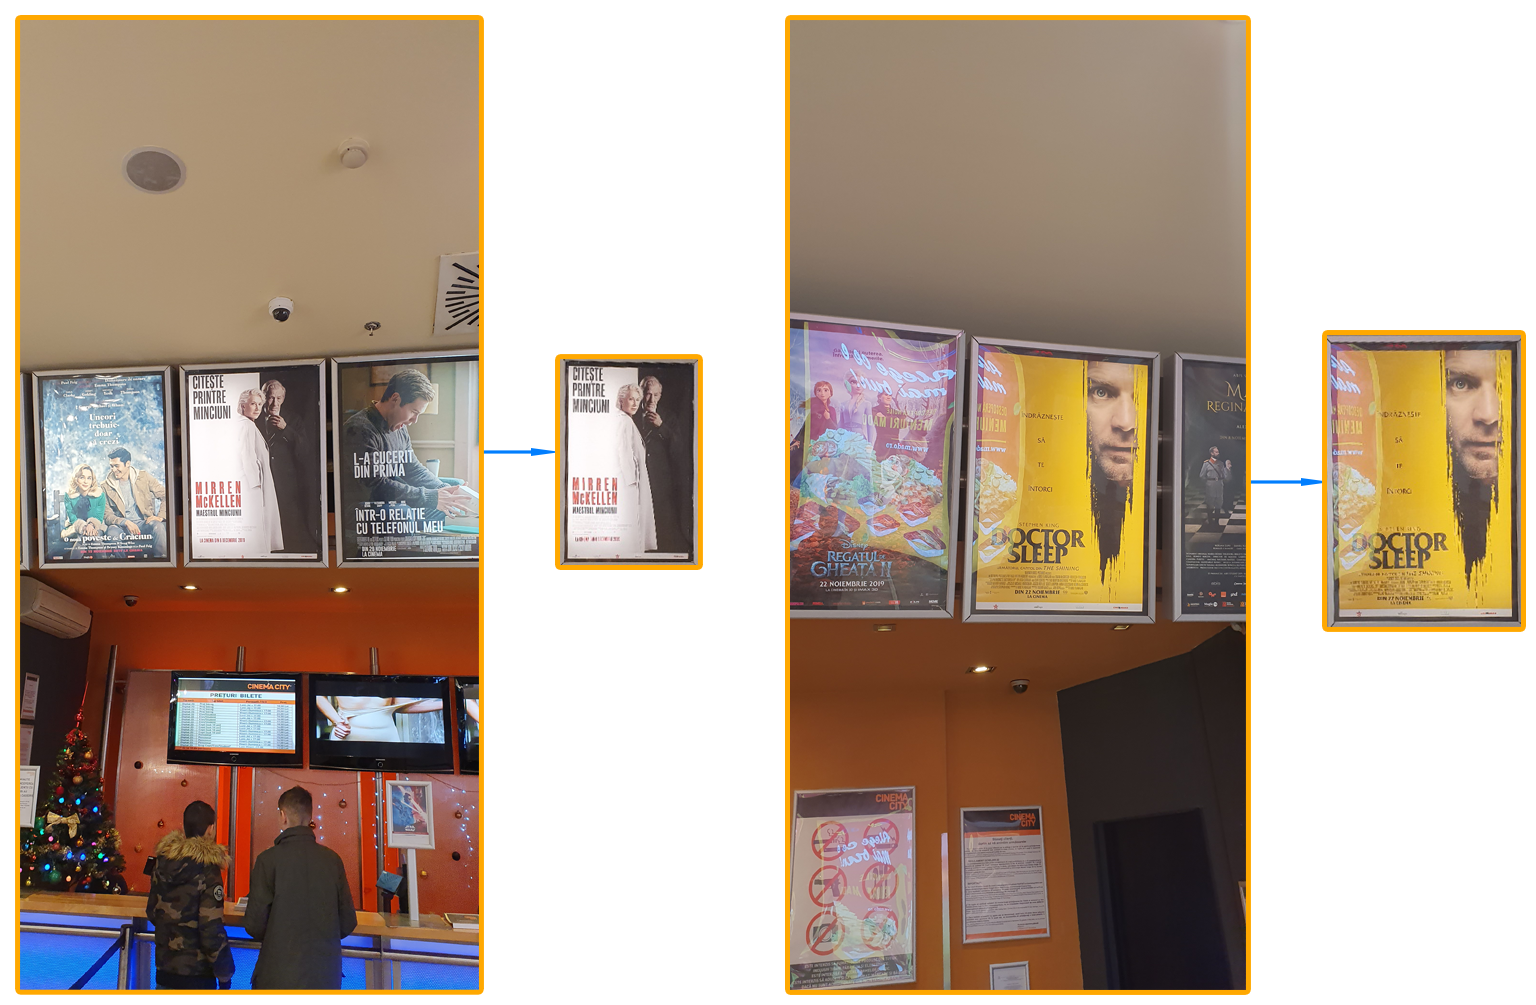
\includegraphics[width=390px]{templateLaTeX-Eng/img/posterdetectiontest.png}
        \caption{\bf Poster detector tests.}
    \end{center}
\end{figure}

The web crawlers have no reason to fail. If a movie is not found in one of the sources, the system will simply return an empty list. The only thing that can compromise the crawlers is that the sources change their web page layout. This will, in turn, require us to re-implement the web crawlers, albeit not completely.

The APIs were tested and their response time was measured. As we can see in the figure below, the OMDb performance is very good. Our Django API has a lesser performance factor due to the fact we didn't optimize it. Also, since it was deployed on the free version of heroku, less resources are allocated to running the web server. We can see that the image search is the most time consuming task. Nevertheless, these are still satisfactory metrics.

 \begin{figure}[H]
    \begin{center}
        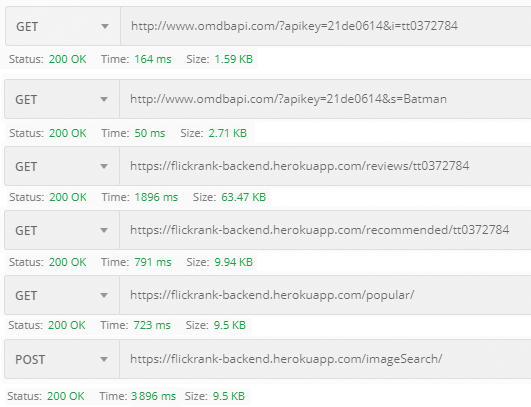
\includegraphics[width=390px]{templateLaTeX-Eng/img/apirequests.png}
        \caption{\bf Poster detector tests.}
    \end{center}
\end{figure}

The performance of the Android application is tied directly to the performance of the APIs. When making calls to the API, loading indicators are shown and the UI is still functional. This helps give the impression of better performance.

Even though Android allows the implementation of unit tests, they are not necessary in this project. Instead, I opted for manual testing in the form of testing it myself, as well as giving the application to numerous users. This process helped me identify many bugs and helped bring the application to a more stable version.

\chapter{User's manual}
\section{Installation Guide}
The only requirement for running and using the FlickRank application is a device running on Android 7 or above. The application is not yet available on the Google Play Store. The only way to install FlickRank is through its apk file. Steps:
\begin{itemize}
    \item Copy the FlickRank.apk file to your Android device.
    \item Open the .apk file.
    \item The OS will warn you about installing applications from unknown sources. In order to use FlickRank, you need to access the phone's settings and allow installation of apks from unknown sources.
    \item When prompted with a dialog asking if you want to install this application, tap "Install".
    \item If prompted by Play Protect, who will try to block the application, tap "Install Anyway".
    \item The application will begin installing. When it is done, you can open the application by tapping "Open".
\end{itemize}
\newpage
 \begin{figure}[H]
    \begin{center}
        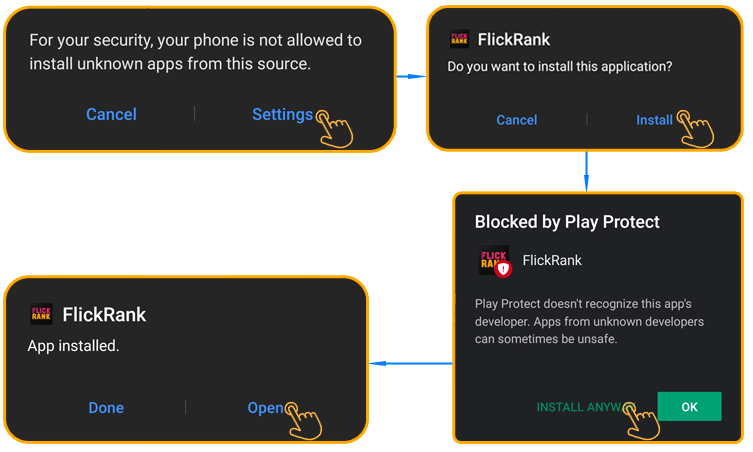
\includegraphics[width=400px]{templateLaTeX-Eng/img/installation.png}
        \caption{\bf Installation steps.}
    \end{center}
\end{figure}

\section{User's Manual}
The main use case of this application would be to search for a movie and read some of its reviews. Steps: 
\begin{enumerate}
    \item Tap the login in with Google button.
    \item Choose the google account you wish to use for FlickRank.
    \item Go to the search tab.
    \item Choose manual search.
    \item Type the title of the movie in the search box.
    \item Choose the desired movie from the search results list.
    \item The movie page will appear.
    \item Scroll down to preview the reviews.
    \item Choose a review and tap on it to read it.
\end{enumerate}

 \begin{figure}[H]
    \begin{center}
        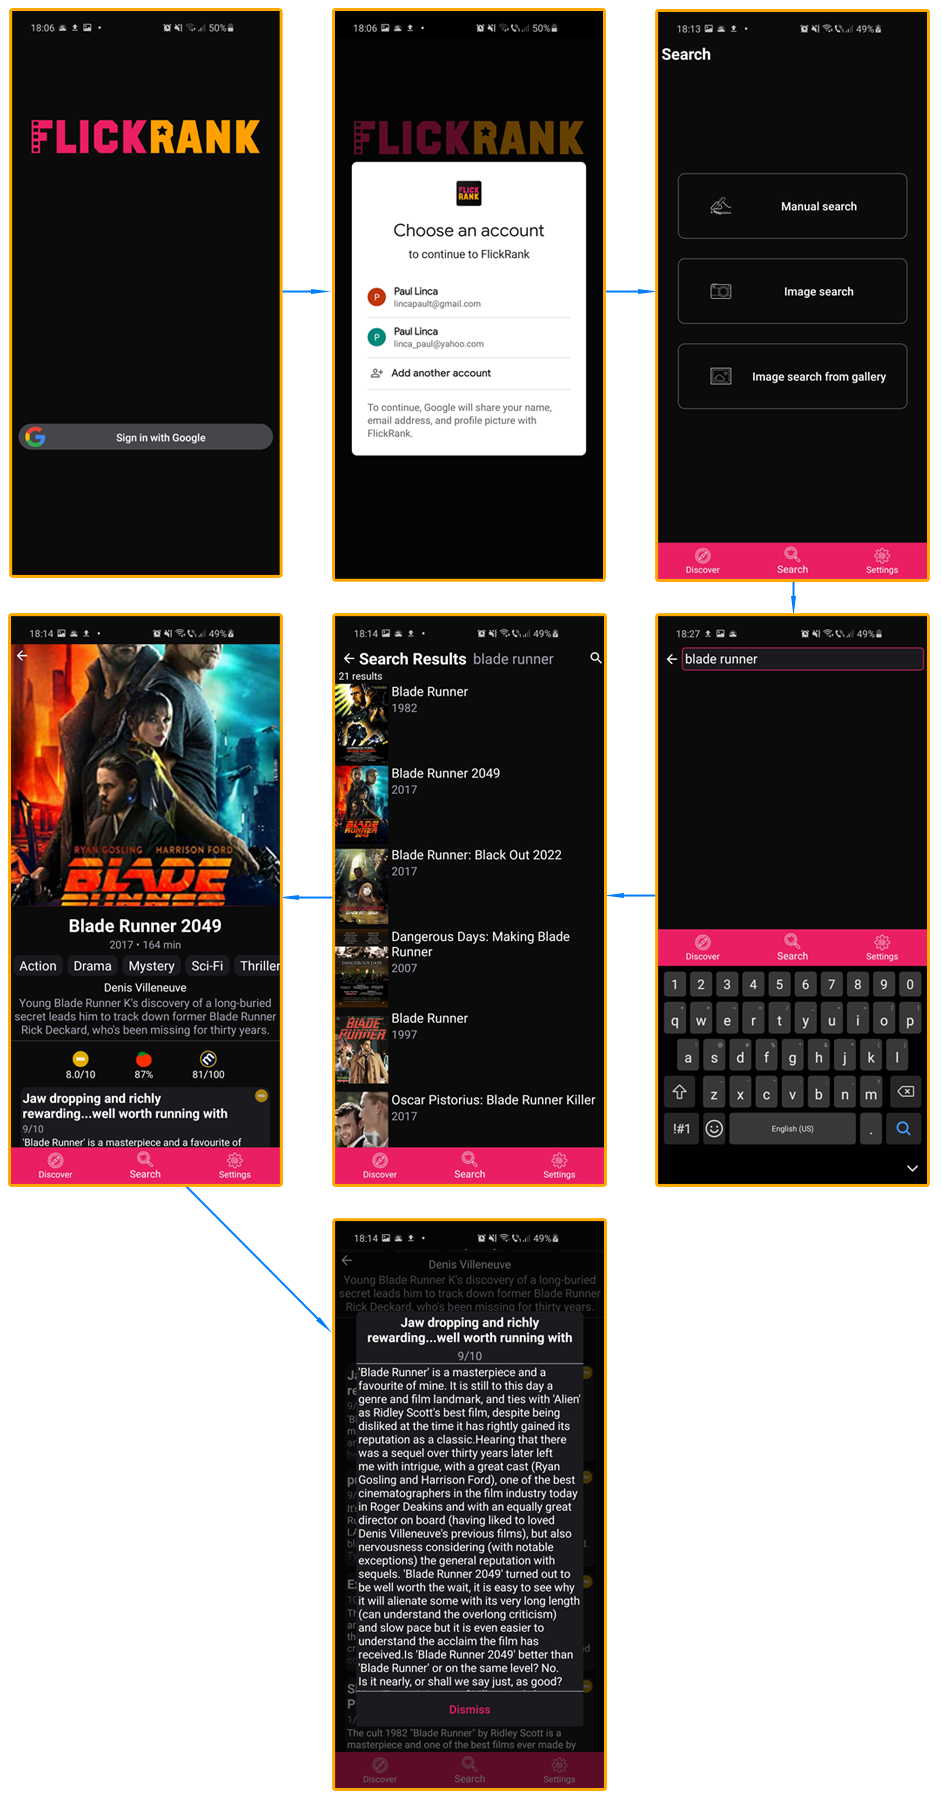
\includegraphics[width=300px]{templateLaTeX-Eng/img/mainusecase.png}
        \caption{\bf Steps for searching for a movie and reading its reviews.}
    \end{center}
\end{figure}

After going thought the main steps mentioned above, some other features can be observed:
\begin{itemize}
    \item Upon returning to the search page, the searched query will appear as a recent search.
    \item The Discover tab will display today's popular movies, a list of the last seen movies within the application and a list of recommendation based on the previously mentioned list.
    \item The setting page provides the options to clear the search history, clear the recently viewed history and log out of the application.
    \item Users can opt for image search in the Search tab by either taking a photo or choosing an existing one from the device's gallery.
\end{itemize}

\begin{figure}[H]
    \begin{center}
        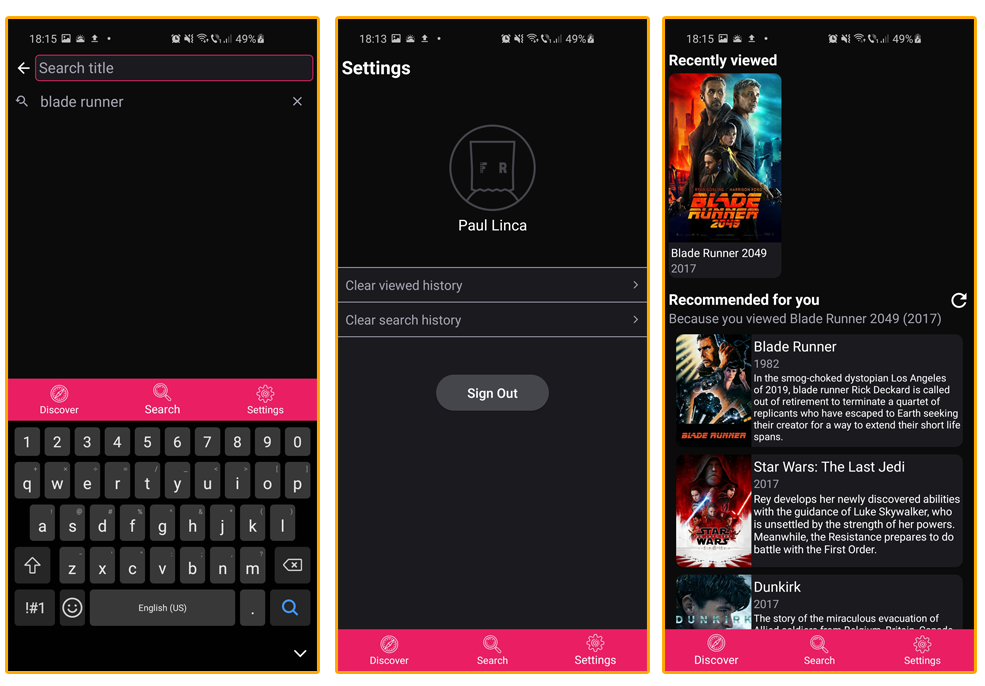
\includegraphics[width=400px]{templateLaTeX-Eng/img/features.png}
        \caption{\bf Depiction of the features mentioned above.}
    \end{center}
\end{figure}

\chapter{Conclusions}
\section{Contribution \& Achievements}
The overall purpose of the project was achieved. The resulted product is an Android application that communicates with several APIs, one of which includes image processing and web scraping functionalities. All these components were developed by me and have turned out great. Since its inception, the project was broken down into sub-goals:
\begin{itemize}
    \item Researched about all the technologies available and all the best practices used to achieve the overall purpose of the project. I used the latest and best documented tools available. 
    \item I learned two new programming languages for me: Python and Kotlin.
    \item I used four new technologies/frameworks: Android Jetpack / AndoridX, BeautifulSoup, Django and Heroku.
    \item Developed an image processing application that takes a photo and detects and identifies a movie poster. While not perfect, developing it proved to be a challenge and taught me a lot.
    \item Created two movie review web crawlers that can work independently and reliably. This opened a new horizon in terms of what applications I could achieve in the future.
    \item Created a web application that contains the two previous applications and exposes them as endpoints.
    \item Deployed the API on Heroku.
    \item Created a state-of-the-art Android application, using the best practices available and putting an accent on the app's architecture.
\end{itemize}

\section{Critical Analysis \& Further Improvements}
The results achieved are satisfactory and align with the initial goals. The developed system has many parts that communicate with each other and each of them is fairly complex. Even so, all the goals were achieved successfully.

That being said, many aspects that can be improved and a lot of additional features that could be added. A lot of these aspects are due to the lack of time. A distribute system like this one usually takes a lot of time to develop and a dedicate team of developers. 

\noindent Things that could be improved:
\begin{itemize}
    \item Improve poster detection by adding more preprocessing steps to remove inconsistencies, noise, glare and other external factors that could lead to a faulty detection.
    \item Improve poster recognition by implementing it using machine learning and neural networks.
    \item Add more web crawlers in order to provide a greater array of sources.
    \item Optimize the API.
    \item Add more authentication options to the Android application, like Facebook auth.
    \item Deploy the application on Google Play.
    \item Provide a more personalized experience to the user by making use of tools like analytics.
\end{itemize}

\begin{thebibliography}{9}

\bibitem{1} 
National Retail Federation
\textit{Convenience and the Consumer}. 
Consumer View Winter, 2020:
\url{https://nrf.com/research/consumer-view-winter-2020}

\bibitem{2} 
 Shanhong Liu,
 \textit{Android - Statistics & Facts}. 
Statista, Jun 2, 2020:
\url{https://www.statista.com/topics/876/android/}

\bibitem{3} 
Stepin Solutions,
 \textit{API Programming : Backbone of Mobile App Development}: 
\url{http://www.stepin-solutions.com/blog/api-programming-backbone-of-mobile-app-development/}

\bibitem{4} 
Salz, P,
 \textit{Monitoring mobile app performance}.
 J Direct Data Digit Mark Pract 15, 219–221 (2014).
\url{https://doi.org/10.1057/dddmp.2014.9}

\bibitem{5} 
Yoel Inbara, Simona Bottib, Karlene Hankoc,
\textit{Decision speed and choice re-gret: When haste feels like waste.}
 Journal of Experimental Social Psychol-ogy, Vol. 47, Issue 3, May 2011.
 
 \bibitem{6} 
Kathleen L. Mosier, Linda J. Skitka,
\textit{Human Decision Makers and Auto-mated Decision Aids: Made for Each Other?}
Automation and HumanPerformance, 1996.

 \bibitem{7} 
Dr. Eugene J. Kelley,
\textit{The Importance of Convenience in Consumer Purchasing.}
First Published July 1, 1958.
\url{https://doi.org/10.1177/002224295802300105}

 \bibitem{8} 
John C. Russ,
\textit{Image Processing.}
Computer-Assisted Microscopy, pp 33-69, ISBN: 978-1-4612-7868-9

 \bibitem{9} 
Ivan Culjak, David Abram, Tomislav Pribanic, Hrvoje Dzapo, Mario Cifrek,
\textit{A brief introduction to OpenCV}
Published in Proceedings of the 35th International Convention MIPRO, 21-25 May 2012. ISBN: 978-953-233-068-7.

 \bibitem{10} 
P. Shopa, N. Sumitha, P.S.K Patra,
\textit{Traffic sign detection and recognition using OpenCV.}
Published in International Conference on Information Communication and Embedded Systems, 27-28 Feb. 2014. ISBN: 978-1-4799-3834-6

\bibitem{11}
Matthew Russell, Scott Fischaber
\textit{OpenCV based road sign recognition on Zynq.}
Published on the 11th IEEE International Conference on Industrial Informatics, 29-31 July 2013, ISBN:  978-1-4799-0752-6.

\bibitem{12}
Guobo Xie and Wen Lu,
\textit{Image Edge Detection Based On Opencv .}
International Journal of Electronics and Electrical Engineering Vol. 1, No. 2, June 2013, ISSN: 2315-4462.

\bibitem{13}
Adrian Kaehler, Gary Bradski,
\textit{Learning OpenCV 3: Computer Vision in C++ with the OpenCV Library.}
O'Reilly Media, Inc., 2016, ISBN: 1491937963, 9781491937969.

\bibitem{14}
OpenCV: Template Matching [Online]\\
\url{https://docs.opencv.org/3.4/de/da9/tutorial\_template\_matching.html}

\bibitem{15}
Anders Hast, Andrea Marchett,
\textit{Rotation invariant feature matching-based on Gaussian filtered log polar transform and phase correlation.}
Published on the 8th International Symposium on Image and Signal Processing and Analysis, 4-6 Sept. 2013, ISBN: 978-953-184-194-8.

\bibitem{16}
J. Clement,
\textit{Global digital population as of April 2020.} Statista, 
\url{https://www.statista.com/statistics/617136}

\bibitem{17}
Chunmei Zheng, Guomei He, Zuojie Peng,
\textit{A Study of Web Information Extraction Technology Based on Beautiful Soup}
School of Information Engineering, China University of Geosciences, Beijing, 100083, China. 
doi: 10.17706/jcp.10.6.381-387

\bibitem{18}
Beautiful Soup documentation [Online]\\
\url{https://www.crummy.com/software/BeautifulSoup/bs4/doc/}

\bibitem{19}
Sally Jo Cunningham, James Littin and Ian H. Witten
\textit{Applications of Machine Learning in Information Retrieval}
Department of Computer Science
University of Waikato
Hamilton, New Zealand

\bibitem{20}
Martin, Robert C,
\textit{Clean architecture : a craftsman's guide to software structure and design}
Boston, MA : Prentice Hall, 2018. - 400 p. ISBN: 9780134494166.

\bibitem{21}
T. Lou,
\textit{A comparison of Android Native App Architecture
: MVC, MVP and MVVM}
Aalto University, Department of Mathematics and Computer Science, 31 Oct 2016.

\bibitem{22}
Neil Smyth,
\textit{Android Studio 3.5 Development Essentials}
eBookFrenzy, 2019

\bibitem{23}
OMDb API,
\url{http://www.omdbapi.com/}

\bibitem{24}
TMDb API,
\url{https://developers.themoviedb.org/3/getting-started/introduction}

\bibitem{25}
IMDb,
\url{https://www.imdb.com/}

\bibitem{26}
Heroku,
\url{https://dashboard.heroku.com/}

\bibitem{27}
Firebase
\url{https://firebase.google.com/}

\end{thebibliography}

\end{document}